
\chapter{Photoassociation : concept and spectroscopy of $^{87}Sr$ calibrated on $^{88}Sr$}
% Centralized path for the theory figures used in this chapter.
\newcommand{\PATheoryFigDir}{Chapitres/Engineering highly entangled system of photoassociated 87Sr atoms/images/Figures_pour_theorie/}
\newcommand{\PATheoryFig}[1]{\PATheoryFigDir#1}
In quantum metrology, a fundamental limit to the precision of a phase parameter $\phi$ measured with $N$ independent particles is the \textbf{Standard Quantum Limit} (SQL), often referred to as the quantum shot noise, defined as $\Delta\phi_{\text{SQL}} = 1/\sqrt{N}$ \cite{pezze_quantum_2014}. For an ensemble of atoms characterized by an effective individual spin $s$ where interferometry is performed on the extreme projection states, this limit scales as $\Delta\phi_{\text{SQL}} = 1/\sqrt{2Ns}$.
Moving toward this goal, the work presented in this chapter focuses on the essential preliminary step: the spectroscopic identification of the molecular states involved in this spin-selective process. At this stage of the experiment, our system is characterized by the resolution of three distinct spectroscopic lines, meaning we are still far from generating collective quantum correlations. However, the precise mapping of these three lines provides the first direct evidence of the underlying molecular structure and the spin-selection rules at play. The objective of this chapter is thus to benchmark the photoassociation mechanism itself, establishing the necessary spectroscopic foundations required for future spin-manipulation and state-purification protocols.\\

This chapter opens with the fundamental concepts of scattering theory required to understand the mechanisms of photoassociation, which drives the evolution of atomic density through one- and two-body loss processes. Next, we present preliminary experimental results obtained with $^{88}\text{Sr}$. Leveraging the well-documented molecular potentials of this bosonic species allows us to benchmark and calibrate our experimental setup. Building upon these foundations, we then focus on the fermionic isotope, $^{87}\text{Sr}$. We provide a detailed presentation of the experimental data, accompanied by a thorough analysis of the technical challenges and systematic issues that could account for the low contrast observed in the molecular lines. Finally, the chapter concludes with a discussion regarding the surprising number of detected lines and their specific profiles, which may hint at the existence of yet unexplained physical phenomena.
\section{Introduction to photoassociation}
\subsection{Scattering theory}
Understanding the PA process necessitates an introduction to scattering theory to define key quantities such as the scattering length and the optical length. These parameters emerge naturally from the asymptotic analysis of the radial Schrödinger equation describing the relative motion of two colliding atoms.

In the study of inter-atomic interactions, the Born-Oppenheimer approximation provides a natural simplification. Due to the large mass ratio between the nuclei and the electrons, the nuclei move on a much slower timescale. One can therefore solve the electronic problem for fixed nuclear positions. The resulting electronic energy curve as a function of the inter-nuclear distance $r$ defines the adiabatic potential $\hat{U}(r)$ experienced by the two atoms. 

Assuming a spherically symmetric potential $\hat{U}(r)$, the treatment of the two-body collision in the center-of-mass frame allows the total relative wavefunction to be factorized into radial and angular parts:
\begin{equation}
    \psi(r, \theta,\phi) = \frac{u_l(r)}{r} Y^m_l(\theta, \phi)
\end{equation}
where the spherical harmonics $Y^m_l(\theta, \phi)$ encode the angular dependence and $l$ denotes the partial wave quantum number. By introducing the reduced mass of the two-atom system $\mu_N = m_{\text{at}}/2$, the Schrödinger equation reduces to a one-dimensional radial equation for each partial wave $l$:

\begin{equation}
    \left( -\frac{\hbar^2}{2\mu_N} \frac{d^2}{dr^2} + \frac{\hbar^2 l(l+1)}{2\mu_N r^2} + \hat{U}(r) \right) u_l(r) = E u_l(r)
    \label{radial equation}
\end{equation}
E the eigenvalue associated to the eigenfunction $u(r)$.
This one-dimensional structure allows a direct analogy with the 1D quantum framework \cite{Landau}. To extract the scattering properties of the system, one studies the asymptotic behavior of the solutions at large distances. Where the inter-atomic potential $\hat{V}(r)$ vanishes, the general solution for $u_l(r)$ takes the form \cite{dalibard_interactions_nodate}:
\begin{equation}
    u_l(r) \xrightarrow{r\to\infty} a_l \sin\left(kr - \frac{l\pi}{2} + \delta_l\right)
    \label{solution at long r}
\end{equation}

where $a_l$ is a normalization factor, $k = \sqrt{2\mu_N E}/\hbar$ is the collision wavenumber, and $\delta_l$ is the phase shift acquired by the $l$-th partial wave due to the short-range interaction potential.

For inter-atomic distances where $1/r^2$ and $V(r)$ are important \cite{dalibard_interactions_nodate} 
\begin{equation}
    u_l(r) \propto r^{l+1} + \frac{a}{r^l}
\end{equation}
$a$ a constant. Then continuity of the wavefunction in the full space imposes a constraint on the phase shifts which at low momenta $k$ that finds:
 \begin{equation}
    \delta_l \propto k^{2l+1}
 \end{equation}

For s-waves ($l=0$), this leads to the definition of the scattering length:
\begin{equation}
    a = -\lim_{k\to 0} \delta_0/k
    \label{scattering length}
\end{equation}

The full wavefunction is recovered by summing over all partial waves. At large distances, this
superposition can be rewritten as an incoming plane wave and an outgoing scattered spherical wave:

\begin{equation}
    \Psi \xrightarrow{r\to\infty} e^{i\mathbf{k}\cdot \mathbf{z}} + f(\theta) \frac{e^{ikr}}{r}
    \label{incoming outcoming scattering wave}
\end{equation}

where $f(\theta)$ is the scattering amplitude which can model both elastic and inelastic collisions and $\theta$ is the angle between the incident and scattered wavevectors. This amplitude expresses for a specific partial wave $l$ as
\begin{equation}
    f_l = \frac{1}{2 i k}(e^{2i\delta_l} -1)
\end{equation}

\begin{figure}
   \centering
   
\includegraphics[width=0.9\linewidth]{Chapitres/Engineering highly entangled system of photoassociated 87Sr atoms/images/Figures_pour_theorie/diffusion_sinus.pdf}
    \caption[fig:scattering\_concept]{The wavefunction $\Psi$ at large inter-atomic distances r behaves as a summation of an incoming plane wave
    and an outgoing spherical wave with attenuated amplitude $f(\theta)$. Here is a representation of this wavefunction for s-wave
    collisions at $l=0$. The scattering occurs at background scattering length $r = a_{bg}$ the distance
    where the elastic collisions properties start to be modified.}
    \label{fig:scattering_concept}
\end{figure}

The assymptotical expression of $\Psi$ and $e^{ikz}$ is expressed in a spherical basis as a sum
over all the partial waves. Then we can give as in \ref{incoming outcoming scattering wave} a decomposition of $\Psi$:
\begin{equation}
    \Psi \simeq \frac{i}{2kr}\sum_{l=0}^{\infty}(2l+1)\left((-1)^l e^{-ikr} - S_l e^{ikr}\right)
    \label{1D schrodinger solution}
\end{equation}

where we identify a spherical part and a scattering term with $S_l = e^{2i\delta_l}$ a coefficient characterising the weight of the inelastic collisions.\\

In the presence of inelastic processes such as photoassociation, the colliding atom pair can be irreversibly lost
from the scattering channel-either by forming a bound molecular
state or by releasing kinetic energy. This loss of flux from the
incoming channel cannot be captured by a purely real phase shift,
as $|S_l|= 1$ implies full conservation of the wavefunction
amplitude. To account for this absorption of flux, $\delta_l$
must be extended to the complex plane, allowing $|S_l| < 1$
and introducing the possibility of inelastic scattering.\\

The associated elastic cross section representing the surface where the scope
of the potential is effective writes as
\begin{equation}
    \sigma_{el} = \frac{\pi}{k^2}\sum_{l=0}^{\infty}(2l+1)|1-S_l|^2
    \label{sigma elastic}
\end{equation}
But we see in equation \ref{1D schrodinger solution} that $|S_l|$ needs to be $<1$ to allow dissipation of the
wavefunction. Defining $\delta_l$ as a complex number satisfies this condition and the inelastic cross section
is

\begin{equation}
    \sigma_{inel} = \frac{\pi}{k^2}\sum_{l=0}^{\infty}(2l+1)(1-|S_l|^2)
    \label{sigma inelastic}
\end{equation}


Then from the condition $\delta_0 << 1$ we deduce an approximated scattering amplitude $S_0$
\begin{equation}
    S_0 = e^{2i\delta_0} \simeq 1 + 2i\delta_0
\end{equation}

Added to the result of \ref{scattering length},
\begin{equation}
     1 + 2i\delta_0 \simeq 1 - 2ika
\end{equation}

Because $\delta_0$ is complex, a direct result of these equations is that we can write a general scattering length as
\begin{equation}
    a = a_{bg} + i a''
\end{equation}

At low temperatures we can re-express equations \ref{sigma elastic} and \ref{sigma inelastic} as
\begin{equation}
    \sigma_{el} = 4\pi|a|^2
\end{equation}
\begin{equation}
    \sigma_{inel} = 4\pi|a''|^2
\end{equation}

As an illustration a usual case of the elastic collisions is atoms in the ground
state. For inelasticity photoassociation is a good example of
dissipative process where two atoms in the ground state are coupled to a molecular state by a laser.
\subsection{PA and complex scattering length}
Photoassociation (PA) is a process in which a pair of colliding free atoms absorbs a photon to form a bound molecule in an excited electronic state. Effectively, because the short-lived molecule quickly decays into deeply bound states or dissociates with high kinetic energy, it escapes the optical trap. Consequently, the bound molecule is typically seen as lost, and the process is perceived as a macroscopic two-body loss effect.

In the atomic pair frame, the electric dipole interaction drives the system from the ground electronic state $\psi_g$ of potential $U_g(r)$ to the excited molecular state $\psi_e$ of potential $U_e(r)$. In the absence of a resonant laser, the internal evolution of the system is purely elastic and expresses as:
\begin{equation}
    i\hbar \frac{d}{dt}
    \begin{pmatrix}
        \psi_g\\
        \psi_e
    \end{pmatrix}
    =
    \begin{pmatrix}
        -\frac{\hbar^2}{2\mu}\nabla^2 + U_g & 0\\
        0 & -\frac{\hbar^2}{2\mu}\nabla^2 + U_e - i\hbar \frac{\Gamma_{mol}}{2}
    \end{pmatrix}
    \begin{pmatrix}
        \psi_g\\
        \psi_e
    \end{pmatrix}.
    \label{elastic evolution equation}
\end{equation}

In the frame of \cite{nicholson_optical_2015} one treat the case when a laser is tuned near a specific vibrational level of the excited potential $U_e(r)$, coupling the free-atom continuum to the bound molecular state, as illustrated in Fig.~\ref{fig:PA_concept}.
\begin{figure}
    \centering
    
\includegraphics[width=0.7\linewidth]{Chapitres/Engineering highly entangled system of photoassociated 87Sr atoms/images/Figures_pour_theorie/Guttridge_PA_process.pdf}
    \caption{Adapted from \cite{guttridge_photoassociation_2019}. General concept of photoassociation: a resonant laser couples a pair of colliding atoms from the free-atom continuum to a bound state of an excited molecular potential. Within this potential, the molecule occupies quantized vibrational states, described by the solutions of the 1D radial Schrödinger equation plotted for each level.}
    \label{fig:PA_concept}
\end{figure}

This coupling introduces inelastic channels into the system. The effective coupled-channel equation becomes:
\begin{equation}
    i\hbar \frac{d}{dt}
    \begin{pmatrix}
        \psi_g\\
        \psi_e
    \end{pmatrix}
    =
    \begin{pmatrix}
        -\frac{\hbar^2}{2\mu}\nabla^2 + U_g & \hbar\Omega/2\\
        \hbar\Omega/2 & -\frac{\hbar^2}{2\mu}\nabla^2 + U_e + \hbar \Delta -i\hbar\frac{\Gamma_{\text{mol}}}{2}
    \end{pmatrix}
    \begin{pmatrix}
        \psi_g\\
        \psi_e
    \end{pmatrix}
    \label{inelastic evolution equation}
\end{equation}
where $\Gamma_{\text{mol}}$ is the natural molecular spontaneous emission linewidth, $\Delta = \omega_e-\omega_L$ is the laser detuning from the excited bound state, and $\hbar \Omega/2$ represents the coherent optical coupling.

This matrix equation shows that the laser creates a bridge between the two manifolds. During a collision, two atoms approaching each other on the ground potential $U_g(r)$ have a non-zero probability to absorb a photon and transition to the excited molecular potential $U_e(r)$. Once populated, this state decays via spontaneous emission at a rate $\Gamma_{\text{mol}}$. To account for this particle loss within the quantum mechanical framework, the molecular decay appears as an imaginary term $-i\hbar\frac{\Gamma_{\text{mol}}}{2}$ in the Hamiltonian matrix. In quantum scattering theory, such an imaginary component acts as a sink that absorbs probability flux, directly translating the physical disappearance of the atoms from the elastic channel.

Since the laser is tuned far from any bare atomic resonance, the excited molecular state remains weakly populated, meaning the atoms spend most of their time interacting on the ground-state potential.
To isolate the response of the excited molecular channel, we expand the closed-channel wavefunction $\psi_e(r)$ onto the bound vibrational eigenstates $\vert{}v_e\rangle$ of the excited Hamiltonian $\hat{H}_e = -\frac{\hbar^2\nabla^2}{2\mu} + U_e(r)$, which satisfy $\hat{H}_e \vert{}v_e\rangle = E_{v_e} \vert{}v_e\rangle$. Projecting the second line of Eq.~\ref{inelastic evolution equation} onto a specific isolated vibrational state $\vert{}v_e\rangle$ yields:
\begin{gather}
E \psi_e = \frac{\hbar \hat{\Omega}}{2}\psi_g + \left(\hat{H}_e + \hbar \Delta - i\hbar \frac{\Gamma_{\text{mol}}}{2} \right)\psi_e\\
\bra{v_e}(E-\hat{H}_e)\psi_e = \bra{v_e}\frac{\hbar\hat{\Omega}}{2}\ket{\psi_g}\\
\psi_e(r) \approx \frac{\left\langle v_e \middle| \frac{\hbar\hat{\Omega}(r)}{2} \middle| \psi_g \right\rangle}{E - E_{v_e} + \hbar\Delta + i\hbar\frac{\Gamma_{\text{mol}}}{2}} v_e(r)
\end{gather}
Substituting this spatial projection back into the ground-state channel (first line of Eq.~\ref{inelastic evolution equation}) yields:
\begin{gather}
    i\hbar\frac{d}{dt}\psi_g = \left(-\frac{\hbar^2\hat{\nabla}^2}{2\mu}+\hat{U}_g\right)\psi_g +\frac{\hbar\hat{\Omega}}{2}\psi_e\\
    \left(E+\frac{\hbar^2\hat{\nabla}^2}{2\mu} - \hat{U}_g\right) \psi_g = \frac{\hbar\hat{\Omega}}{2} \psi_e\\
    \left(E+\frac{\hbar^2\hat{\nabla}^2}{2\mu} - \hat{U}_g\right) \psi_g = \frac{\hbar\hat{\Omega}}{2} \frac{\frac{\hbar\hat{\Omega}}{2}\ket{v_e}\bra{v_e}\frac{\hbar\hat{\Omega}}{2}}{E-E_{v_e} + \hbar\Delta + i\hbar\frac{\Gamma_{\text{mol}}}{2}}\psi_g
\end{gather}
\begin{equation}
\left(-\frac{\hbar^2\hat{\nabla}^2}{2\mu} + \hat{U}_g(r) + \hat{V}\right)\psi_g(r) = E \psi_g(r)
\label{psi e dans psi g}
\end{equation}
One want to isolate the term that concerns the ground state to observe the modifications of it from the coupling to the molecular state. Then by projecting \ref{psi e dans psi g} we define $\langle\hat{V}\rangle$ as:
\begin{equation}
\langle \psi_g | \hat{V} | \psi_g \rangle = \frac{\left| \left\langle v_e \middle| \frac{\hbar\hat{\Omega}(r)}{2} \middle| \psi_g \right\rangle \right|^2}{E - E_{v_e} + \hbar\Delta + i\hbar\frac{\Gamma_{\text{mol}}}{2}}
\label{V_opt}
\end{equation}
Following Bohn and Julienne \cite{bohn1997_prospects}, one can define the stimutaled rate $\Gamma_{stim}$ from $\ket{v_e}$ to $\ket{\psi_g}$ by the Fermi-Golden rule as
\begin{equation}
    \Gamma_{stim} = 2\pi\left(\frac{2\pi I}{c}\right)d^2\left| \bra{v_e} \psi_g \rangle \right|^2
\end{equation}

with I the laser intensity, c the light velocity and d the transition dipole moment. On equation \ref{V_opt} the $\frac{\hbar\hat{\Omega}(r)}{2}$ comes from the dipolar interaction of the atoms with the eletric field $\vec{E}$
of the laser, also expressing as $\frac{\hbar\hat{\Omega(r)}}{2} = \vec{d}.\vec{E}$. One identify the numerator of \ref{V_opt} as the stimulated linewidth $\Gamma_{stim}$. This rate depends on the \textbf{Franck-Condon factor} that 
is the overlape between the ground state wavefunction and the excited molecular state.\\


Also integrating the optical potential $\hat{V}$ within the asymptotic boundary conditions for $r \to \infty$ modifies the scattering phase shift, leading to the complex scattering length $a(\Delta)$:

\begin{equation}
a(\Delta) = a_{\text{bg}} + \frac{l_{\text{opt}}\Gamma_{\text{mol}}}{\Delta + i\frac{\Gamma_{\text{mol}}}{2}}
\label{a(delta)}
\end{equation}

where $a_{\text{bg}}$ is the real background scattering length representing native elastic collisions \cite{yan_controlling_2013}. The parameter $l_{\text{opt}}$ is the temperature-independent optical scattering length, which encapsulates the strength of the light-induced interaction and scales strictly linearly with the laser intensity $I$. The light-induced stimulated linewidth $\Gamma_{\text{stim}}(k)$ accounts for the laser coupling and scales linearly with the wavevector $k$ at low temperature according to \cite{tiesinga2005measurement}:
\begin{equation}
    \Gamma_{\text{stim}}(k) = 2 k l_{\text{opt}} \Gamma_{\text{mol}}
    \label{eq:gamma_stim_blatt}
\end{equation}
where $l_{\text{opt}}$ is the temperature-independent \textbf{optical length}, a central parameter characterizing the strength of the light-matter coupling which scales linearly with the laser intensity $I$.

To distinguish how the laser independently alters the elastic interactions and the loss mechanisms, we multiply the resonant fraction in Eq.~\ref{a(delta)} by the complex conjugate of its denominator. This algebraic separation successfully decouples the scattering length into its real (dispersive) and imaginary (absorptive) components, $a(\Delta) = a_{\text{bg}} + \delta a(\Delta) + i a''(\Delta)$:
\begin{equation}
    a(\Delta) = a_{\text{bg}} + \frac{l_{\text{opt}}\Gamma_{\text{mol}}\Delta}{\Delta^2 + \left(\frac{\Gamma_{\text{mol}}}{2}\right)^2} - i \frac{l_{\text{opt}}\Gamma_{\text{mol}}\frac{\Gamma_{\text{mol}}}{2}}{\Delta^2 + \left(\frac{\eta \Gamma_{\text{mol}}}{2}\right)^2}
\end{equation}
The real light-induced shift $\delta a(\Delta)$ governs the modification of the elastic properties of the gas, whereas the imaginary part $a''(\Delta)$ directly quantifies the rate of inelastic two-body losses.
\subsection{General scaling laws for PA}
To connect this microscopic scattering amplitude to observable experimental quantities, one must translate these individual collision events into a population decay that writes as:
\begin{equation}
    \frac{dN}{dt} = -\beta(T) N^2 - \Gamma N
\end{equation}
where $\beta(T)$ is related to the two-body loss rate $K_2$ and $\Gamma$ is the one-body loss rate that depends experimentally mostly on the vacuum quality.\\

In quantum scattering theory, the fundamental two-body loss rate coefficient $K_2(k)$ is directly driven by the absorptive (imaginary) part of the scattering length $a''$ derived from Eq.~\ref{V_opt}:
\begin{equation}
    K_2(k) = \frac{8\pi\hbar}{m_{\text{at}}} a''(k, \Delta)
    \label{eq:K2_a_second}
\end{equation}

Grounded on the systematic study of optical Feshbach resonances by Blatt et al. \cite{blatt_systematic_2011}, substituting the expression of $a''$ into Eq.~\ref{eq:K2_a_second} yields the complete expression for the loss coefficient as a function of the collision wavevector $k$:

\begin{equation}
    K_2(k) = \frac{8\pi \hbar}{m_{\text{at}} k} \times \frac{\Gamma_{\text{mol}} \Gamma_{\text{stim}}(k)}{\Delta^2 + \frac{1}{4}\big(\Gamma_{\text{mol}} + \Gamma_{\text{stim}}(k)\big)^2}
    \label{K2 complet Blatt}
\end{equation}

where $m_{\text{at}}$ is the atomic mass, $\Delta = \omega_{\text{L}} - \omega_{\text{mol}}$ is the laser detuning from the molecular resonance, and $\Gamma_{\text{mol}}$ is the natural molecular linewidth.

While $K_2$ characterizes the fundamental two-body collision process, the experimentally observed decay coefficient $\beta$ depends on the spatial density distribution of the atomic cloud of width $\sigma_x, \sigma_y, \sigma_z$. The relation between $K_2$ and $\beta$ is derived by integrating the local loss over a Gaussian density profile:
\begin{gather}
\frac{dN(t,T)}{dt} = -K_2 \iiint n^2(x,y,z,t,T) \, d^3r \label{eq:3.24} \\[1.5ex]
\text{with } n(x,y,z,t,T) = n_0 \exp\left( -\frac{x^2}{2\sigma_x(T)^2} - \frac{y^2}{2\sigma_y(T)^2} - \frac{z^2}{2\sigma_z(T)^2} \right) \label{eq:3.25} \\[1.5ex]
\text{and } n_0 = \frac{N(t,T)}{(2\pi)^{3/2}\sigma_x(T)\sigma_y(T)\sigma_z(T)} \label{eq:3.25bis} \\[1.5ex]
\frac{dN(t,T)}{dt} = -K_2 \frac{N(t,T)^2}{2\sqrt{2}V_{\text{e}}(T)} \equiv -\beta(T) N(t,T)^2 \label{eq:3.26} \\[1.5ex]
\text{where } V_{\text{e}}(T) = (2\pi)^{3/2} \sigma_x(T) \sigma_y(T) \sigma_z(T) \label{eq:3.27} \\[1.5ex]
\text{Then } \beta(T) = \frac{K_2}{2\sqrt{2}V_{\text{e}}(T)} \label{eq:3.28}
\end{gather}
consistent with the definitions found in \cite{han_photoassociation_2018}.

For low temperatures, we neglect the contribution of the wavevector since $k \to 0$. In this threshold regime, the light-induced linewidth becomes negligible compared to the natural molecular width ($\Gamma_{\text{stim}}(k) \ll \Gamma_{\text{mol}}$). On resonance ($\Delta = 0$), substituting Eq.~\ref{eq:gamma_stim_blatt} into Eq.~\ref{K2 complet Blatt} allows the wavevector $k$ to cancel out from the prefactor, and the microscopic PA rate coefficient simplifies to:
\begin{equation}
    K_2 = \frac{16h}{m_{\text{at}}}l_{\text{opt}}
\end{equation}
This fundamental result demonstrates that at low temperatures, the maximum photoassociation rate becomes independent of the temperature and scales purely linearly with the laser intensity $I$ through its dependence on $l_{\text{opt}}$. Structurally, $K_2$ is maximized when the ground- and excited-state wavefunctions exhibit maximum overlap at the Condon radius. In a classical picture, this distance corresponds to the turning point where the colliding atoms spend the most time, maximizing the transition probability.

Finally, by combining Eq.~\ref{eq:3.28} and the low-temperature limit of $K_2$, we obtain the total macroscopic evolution equation of the trapped population:
\begin{equation}
    \frac{dN}{dt} = -\frac{4\sqrt{2} h }{V_{\text{e}} m_{\text{at}}}l_{\text{opt}}N^2 - \Gamma N
\label{one and two body losses equation}
\end{equation}
which highlights that the global loss process is driven by the tunable optical length $l_{\text{opt}}$ and enhanced by the peak atomic density $n_0 \propto 1/V_{\text{e}}$. 

\subsection{Handling multiple molecular potentials}
So far, the photoassociation (PA) process has been presented assuming a simplified picture with a single excited-state molecular potential $U_e$. However, the molecules created via PA exhibit a rich internal structure, making the identification of accessible excited states essential for predicting and optimizing the loss rate coefficient $\beta(T)$.

Unlike atomic spectroscopy, where selecting target states is straightforward, identifying specific molecular target states is significantly more involved due to the dense coexistence of multiple potential energy curves. Following the Born-Oppenheimer approximation, the fast electronic motion decouples from the slower nuclear motion. Each distinct molecular electronic configuration—labeled by its set of molecular quantum numbers—gives rise to an adiabatic potential energy curve $U_e(r)$. Determining these curves $U_e(r)$ is crucial, as they dictate the bound-state wavefunctions $\psi_e(r)$ and govern the overall PA dynamics.

\subsubsection{Symmetry constraints and Pauli exclusion principle}
In ultracold gases, ground-state collisions occur predominantly in the $s$-wave regime ($R_i = 0$), as higher partial waves ($l > 0$) are reflected by the centrifugal barrier before reaching the short-range interaction region. For fermionic $^{87}\text{Sr}$ atoms, Fermi-Dirac statistics impose a overall antisymmetric wavefunction $\ket{\Psi}$ under nuclear permutation. 

For two identical atoms A and B with spatial states $\ket{\beta_1}$ and $\ket{\beta_2}$, the total molecular wavefunction is expressed as:
\begin{equation}
    \ket{\Psi} = \left(\ket{\beta_1}_A \ket{\beta_2}_B - \rho \times p \ket{\beta_1}_B \ket{\beta_2}_A\right) \otimes \ket{\phi}
    \label{wavefunction parity}
\end{equation}
where $\ket{\phi}$ represents the total nuclear spin wavefunction. Since $s$-wave collisions ($R_i = 0$) feature a symmetric spatial wavefunction, Pauli's principle mandates that the ground-state nuclear spin wavefunction $\ket{\phi}$ must be antisymmetric. Because electric dipole ($E1$) transitions act purely on electronic and spatial degrees of freedom, the nuclear spin acts as a spectator; hence, \textbf{$\ket{\phi}$ remains antisymmetric throughout the PA process.}

Following \cite{reichenbach_optical_nodate}, $\rho = p_1 p_2$ denotes the product of the intrinsic electronic parities of the two isolated atoms, while $p = (-1)^R$ reflects the rotational parity associated with the \textbf{molecular rotational quantum number $R$.}

\begin{figure}
    \centering
    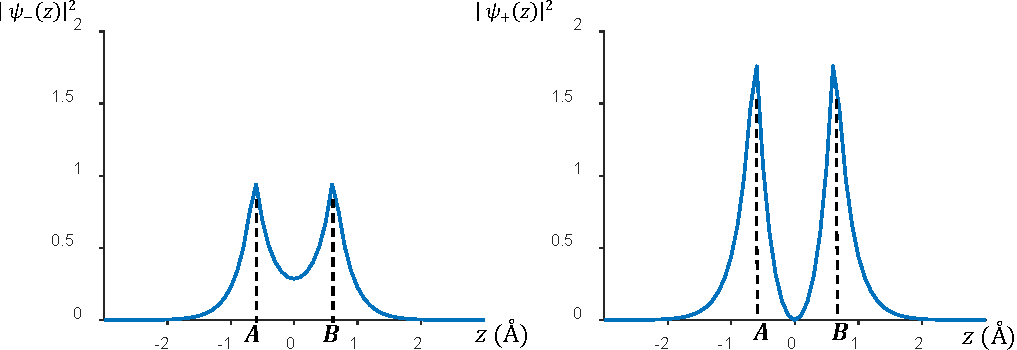
\includegraphics[width=1\linewidth]{Chapitres/Engineering highly entangled system of photoassociated 87Sr atoms/images/Figures_pour_theorie/proba_presence.pdf}
    \caption[Gerade/ungerade electronic symmetry]{Gerade ($g$) and ungerade ($u$) spatial electronic wavefunctions for electrons orbiting nuclei A and B. Left: Square modulus $\left|\psi_-(z)\right|^2$ for an ungerade state, showing a non-zero probability density between the two nuclei. Right: For a gerade state, the electronic probability density vanishes at the midpoint between the nuclei.}
    \label{fig:u-g symmetry}
\end{figure}

\subsubsection{Angular momentum coupling and state enumeration}
Spin-orbit coupling plays a dominant role in shaping the excited molecular structure near the $^1\text{S}_0 - {}^3\text{P}_1$ intercombination asymptote. The total angular momentum of the molecule is defined by $T = R + F = R + I + J$, where $F = f_1 + f_2$ is the coupled atomic angular momentum, $J = j_1 + j_2$ is the total electronic angular momentum, and $R$ is the rotational angular momentum.

Along the internuclear axis, the projection of the electronic angular momentum is quantified by:
\begin{equation}
    \Omega = \Lambda + \Sigma
\end{equation}
where $\Lambda$ and $\Sigma$ represent the internuclear projections of the orbital and spin angular momenta, respectively. Because spin-orbit interaction is strong relative to rotational coupling at short to intermediate ranges, the molecule is appropriately described within Hund's case (c) framework (see Fig.~\ref{fig:hund}), where $\Omega$ remains a good quantum number.

\begin{figure}[H]
    \centering
    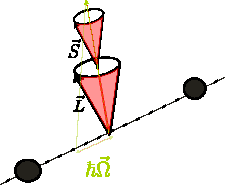
\includegraphics[width=0.7\linewidth]{Chapitres/Engineering highly entangled system of photoassociated 87Sr atoms/images/Figures_pour_theorie/hund_case_c.pdf}
    \caption[Hund's case (c) coupling scheme]{Hund's case (c) coupling scheme, where strong spin-orbit interaction couples the total electronic angular momentum to the internuclear axis with projection $\hbar \Omega$. In most ultracold photoassociation scenarios, the rotational quantum number is low ($R = 0, 1$).}
    \label{fig:hund}
\end{figure}

To determine the accessible target molecular states, we analyze the parity requirements in both initial and final asymptotes:

\begin{itemize}
    \item \textbf{Ground collisional state ($^1\text{S}_0 + {}^1\text{S}_0$):}\\
    Both atoms share identical, even electronic parity ($p_1 = p_2 = +1$), giving $\rho = +1$. To maintain an overall antisymmetric wavefunction with an antisymmetric spin state $\ket{\phi}$, we require $\rho \times p = +1$. This implies $p = +1$, which restricts ground $s$-wave collisions to even rotational numbers ($R_i = 0, 2 \dots$).
    
    \item \textbf{Excited molecular state ($^1\text{S}_0 + {}^3\text{P}_1$):}\\
    The asymptotic electronic parities are opposite ($p_1 = +1, p_2 = -1$), leading to a constant electronic parity product $\rho = -1$. Because the nuclear spin state remains antisymmetric, the Pauli constraint $\rho \times p = +1$ requires $p = -1$. Consequently, the excited molecular states accessible from $s$-wave collisions must feature odd rotational quantum numbers ($R_f = 1, 3, 5 \dots$).
\end{itemize}

Applying these selection rules to $^{87}\text{Sr}$ atoms photoassociated in the $F = 11/2$ manifold (with $f_1 = 9/2$ for $^1\text{S}_0$ and $f_2 = 11/2$ for $^3\text{P}_1$), the electronic angular momentum $J = 1$ couples with nuclear spin to yield total atomic angular momenta $F \in \{1, 2, \dots, 10\}$. Combining $F$ with the allowed odd rotational modes ($R_f = 1, 3, 5\dots$) and taking into account electric dipole selection rules ($|\Delta T| \le 1$ with $T=0 \not\rightarrow T=0$), the accessible final states $T^f$ satisfy:
\begin{align}
\text{For } R_f=1, &\quad T^f \in \{1, 2, \dots, 10\}\\
\text{For } R_f=3, &\quad T^f \in \{1, 2, \dots, 10\}\\
\text{For } R_f=5, &\quad T^f \in \{1, 2, \dots, 10\}
\end{align}
\subsubsection{Effective Hamiltonian and Potential Modeling}

Taking into account the hyperfine-induced mixing between $g$ and $u$ electronic manifolds ($0_u, 1_u, 0_g, 1_g$) at long range—analogous to observations in $^{173}\text{Yb}$ \cite{han_photoassociation_2018}—we estimate a total of approximately **981 accessible $(R_f, T^f)$ molecular configurations**. This massive density of states illustrates the extreme complexity of the excited molecular spectrum to be mapped experimentally.

\begin{figure}[H]
    \centering
    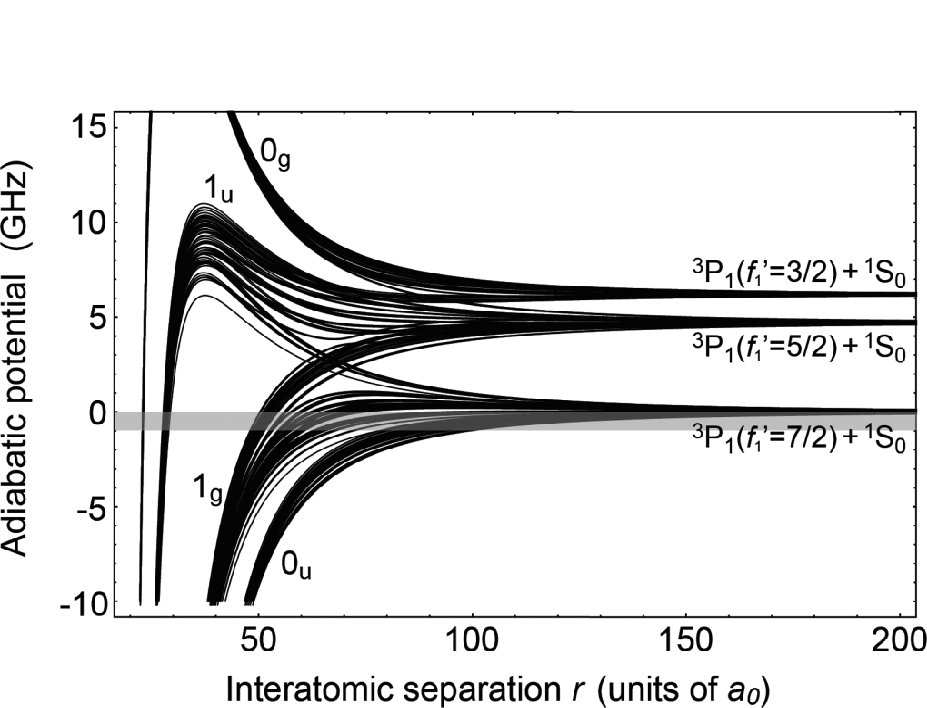
\includegraphics[width=0.8\linewidth]{Chapitres/Engineering highly entangled system of photoassociated 87Sr atoms/images/Figures_pour_theorie/ytterbium.pdf}
    \caption[Density of molecular potentials for $^{173}\text{Yb}$]{Density of molecular potentials for $^{173}\text{Yb}$ with three hyperfine states, giving rise to numerous triplets of quantum numbers $(T, F, R)$. The spectral lines are identified as $S_{u/g}$, where $S$ is the total orbital momentum projection of the molecule and $u/g$ denotes the electronic parity (see Fig.~\ref{fig:u-g symmetry}).}
    \label{fig:pa-ytterbium-potentials}
\end{figure}

The high density of states expected for $^{87}\text{Sr}$ makes spectral assignment particularly challenging. To move beyond a statistical estimation and accurately predict the energy levels of these 981 configurations, precise modeling of the molecular interaction is required. This involves describing the coupling between the rotation of the nuclear frame, the electronic degrees of freedom, and the hyperfine structure.

Following the molecular picture introduced in Section~3.1.1, the energy of these states is governed by the total Hamiltonian $\hat{H}$, which for a Sr--Sr system can be expressed as:
\begin{equation}
    \hat{H} = \frac{\hat{p}_r^2}{2\mu} + \frac{\hbar^2}{2\mu r^2} \hat{R}^2 + \hat{U}_{\text{BO}} + \hat{H}_{\text{hf}}
    \label{eq:general_hamiltonian_molecule}
\end{equation}
where higher-order electronic interactions have been neglected depending on the relevant Hund's case. For $^{87}\text{Sr}$, the Born-Oppenheimer potential $\hat{U}_{\text{BO}}$ is approximated using a long-range expansion similar to $^{173}\text{Yb}$:
\begin{equation}
    \hat{U}_{\text{BO}}(r) = -\frac{C_6}{r^6} \left( 1 - \frac{\sigma^6}{r^6} \right) - s \frac{C_3^{\Omega}}{r^3}
    \label{eq:sr_potential}
\end{equation}
where $s = +1$ and $s = -1$ correspond to $g$ and $u$ potentials, respectively.

The atomic hyperfine Hamiltonian $\hat{H}_{\text{hf}}$ acts solely on the $^3\text{P}_1$ atom (with nuclear spin $i_1 = 9/2$ and electronic angular momentum $j_1 = 1$), as the ground-state $^1\text{S}_0$ atom has $j_2 = 0$ and thus no hyperfine interaction:
\begin{equation}
    \hat{H}_{\text{hf}} = A \, (\mathbf{i}_1 \cdot \mathbf{j}_1) + B \, \frac{3(\mathbf{i}_1 \cdot \mathbf{j}_1)^2 + \frac{3}{2}(\mathbf{i}_1 \cdot \mathbf{j}_1) - i_1(i_1+1) j_1(j_1+1)}{2 i_1 (2 i_1 - 1) \, 2 j_1 (2 j_1 - 1)}
\end{equation}
where $A$ and $B$ are the magnetic dipole and electric quadrupole hyperfine constants, respectively.

Among these potential curves, approximately 80 bound internal states were experimentally identified for $^{173}\text{Yb}$ \cite{han_photoassociation_2018}. Atom-loss spectra, recorded as a function of PA laser detuning, reveal the position of bound states relative to the atomic resonance $|^1\text{S}_0, F=5/2\rangle \to |^3\text{P}_1, F=7/2\rangle$. Near this threshold, atoms are illuminated for $30\,\text{ms}$ at low intensity ($I = 37\,\text{mW/cm}^2$) to avoid power broadening, resolving bound states closest to the dissociation limit. At larger red detunings, higher laser power and optimized exposure times are used to maximize signal depth.

Theoretically, these experimental loss lines are assigned by computing the eigenvalues of the effective Hamiltonian and adjusting parameters such as $C_n$ coefficients to match observed vibrational levels. Several semi-classical tools aid this assignment: the WKB approximation describes the near-threshold bound states, while LeRoy-Bernstein scaling predicts the spacing of consecutive vibrational lines near the dissociation limit without requiring detailed short-range potential data. Finally, mass scaling across strontium isotopes \cite{borkowski_mass_2014} serves as a robust benchmark to cross-check these energy assignments.
\subsection{Internal energy states}
\subsubsection{WKB approximation}

The Wentzel-Kramers-Brillouin (WKB) approximation is a semi-classical method used to estimate the 
vibrational eigenvalues of a diatomic system. By modeling the interatomic potential, the position 
of a first bound state can be determined, which subsequently enables the deduction of the following 
vibrational levels.

In this approach, the wavefunction is assumed to take the form of a modified plane wave 
$\psi(x) = \frac{C}{\sqrt{k(x)}}e^{i\int_{x_0}^{x} k(x') dx'}$. These waves are solutions 
to the one-dimensional Schrödinger equation for two particles with reduced mass $\mu$ and 
eigenenergy $E$:

\begin{equation}
    -\frac{\hbar^2}{2\mu}\frac{d^2\psi}{dx^2} + U(x)\psi = E\psi
    \label{eq:schrodinger_1d}
\end{equation}

This leads to the expression of the local wavevector $k(x)$:
\begin{equation}
    k(x) = \frac{p(x)}{\hbar} = \frac{\sqrt{2\mu(E-U(x))}}{\hbar}
\end{equation}

The validity of this approximation is governed by the condition $\frac{d\lambda}{dx} \ll 1$, 
implying that the local de Broglie wavelength must vary slowly compared to the scale of the 
atoms' motion. This can be explicitly rewritten in terms of the potential gradient:

\begin{equation}
    \left| \frac{\mu \hbar \frac{dU}{dx}}{\left[2\mu(E-U(x))\right]^{3/2}} \right| \ll 1
    \label{eq:wkb_validity}
\end{equation}

This expression highlights two critical regimes where the semi-classical approach fails. 
First, near the classical turning points where $E \approx U(x)$, the kinetic 
energy vanishes and the wavelength diverges. Second, at short internuclear distances
(Region I in Fig. \ref{fig:pa-sakurai-wkb}), the steepness of the repulsive wall $|dU/dx|$ 
becomes too large for the atoms to follow the potential variations adiabatically. In these 
regions, connection formulas, typically using Airy functions, are required to match the 
solutions across the turning points.

\begin{figure}[H]
    \centering
    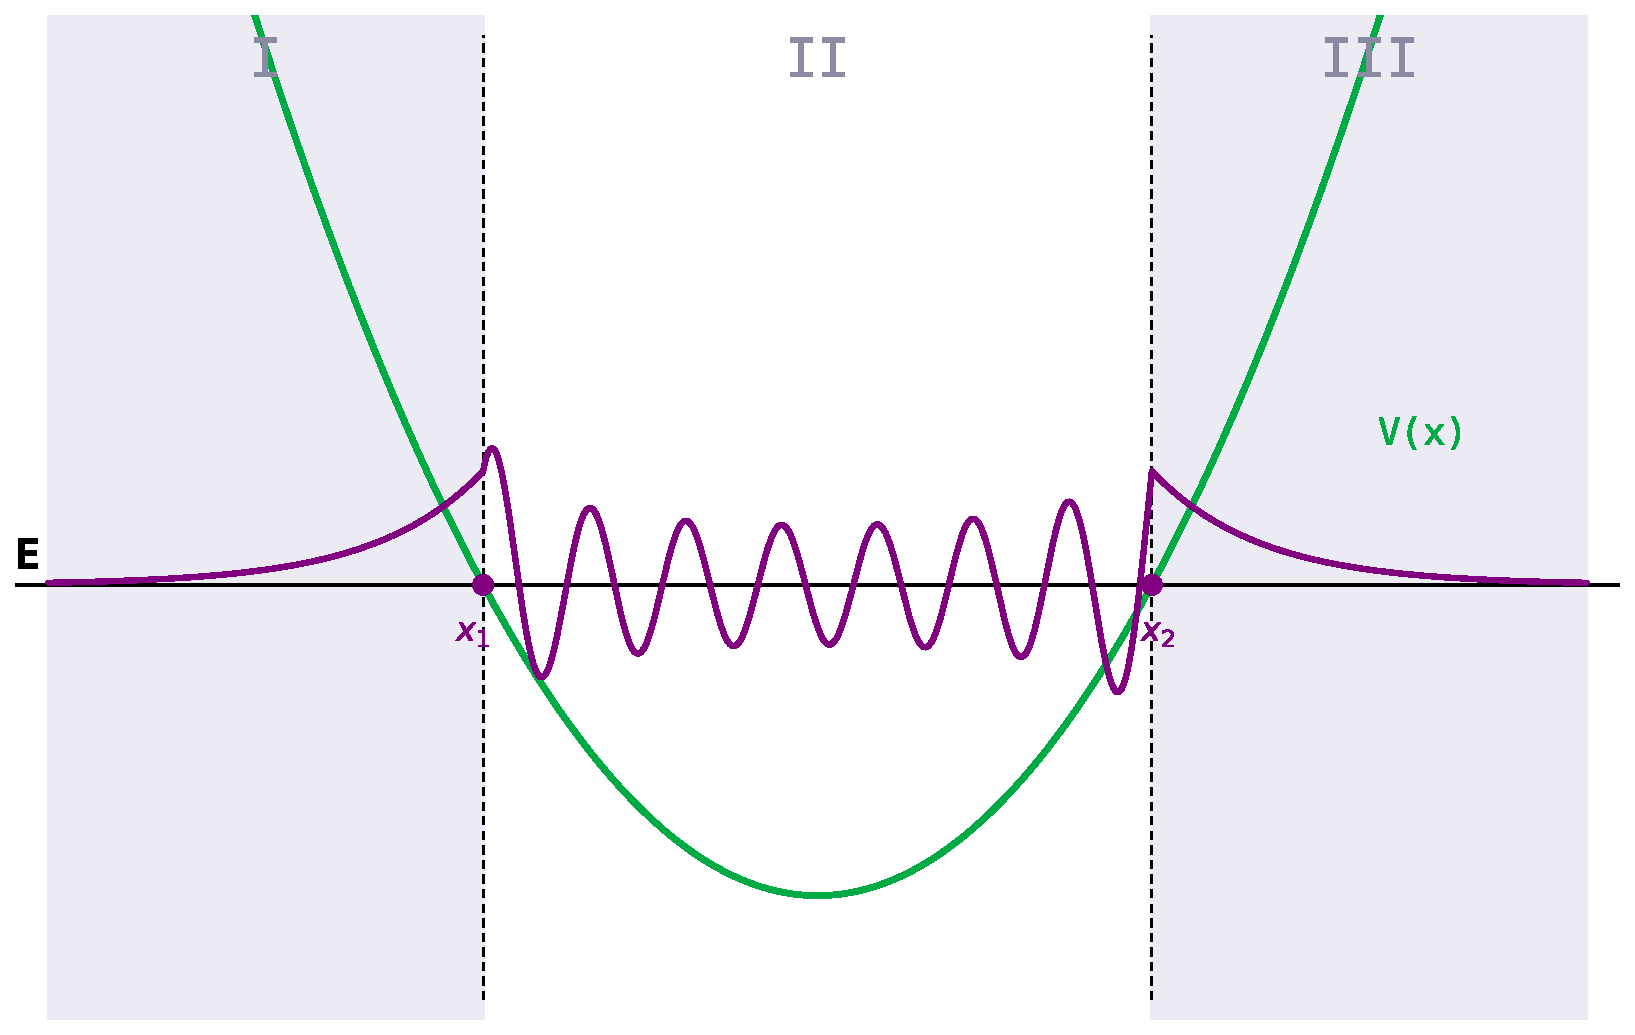
\includegraphics[width=0.8\linewidth]{Chapitres/Engineering highly entangled system of photoassociated 87Sr atoms/images/Figures_pour_theorie/WKB_sakurai.pdf}
    \caption[fig:pa-sakurai-wkb]{Semi-classical approximation in an interatomic potential 
    $U(x)$. The energy level $E$ intersects the potential at the turning points $x_1$ and 
    $x_2$. In the classically allowed Region II, the wavefunction oscillates with an amplitude 
    proportional to $1/\sqrt{k(x)}$. In the forbidden Regions I and III, the wavefunction is 
    evanescent.}
    \label{fig:pa-sakurai-wkb}
\end{figure}

At positions $x=x_1$ and $x_2$, the momentum reaches zero and becomes imaginary as the energy 
level $E$ crosses the potential $U(x)$. In the classically forbidden regions I and III, the 
wavefunction is evanescent and characterized by the decay constant $\kappa(x) = \sqrt{2\mu(U(x)-E)}/\hbar$. 
Around the turning points, it is standard to linearize the potential to connect the oscillatory 
and evanescent solutions. Region I is generally not studied in detail for photoassociation since 
the repulsive wall of the potential is extremely steep and diverges at very short distances.

To ensure a physical stationary state, the phase accumulated by the wave as it reflects between 
the barriers at $x_1$ and $x_2$ must satisfy a quantization condition. By ensuring the continuity 
of the solutions over $[0, +\infty[$, the phase integral must follow:
\begin{equation}
    \int_{x_1}^{x_2} k(x)dx = \left(n+\frac{1}{2}\right)\pi
    \label{eq:wkb_quantization}
\end{equation}

This formula, known as the Bohr-Sommerfeld quantization condition, enables the identification of 
the discrete energy eigenvalues $E_n$ that satisfy the integral. these values correspond to the 
vibrational states of the molecular potential.

\subsubsection{Leroy-Bernstein scaling}


The LeRoy-Bernstein scaling law builds upon the WKB approximation to identify the position of the 
high-lying vibrational states near the dissociation limit. This model is particularly powerful as 
it relies solely on the long-range behavior of the potential, bypassing the need for a detailed 
description of the complex short-range interactions. 

Near the dissociation limit $D_e$, occurring at large internuclear distances $r$, the potential 
can be approximated by its leading long-range term:
\begin{equation}
    U(r) \approx D_e - \frac{C_n}{r^n}
\end{equation}

where $C_n$ is the long-range coefficient (typically $n=6$ for Van der Waals or $n=3$ for resonant 
dipole-dipole interactions). For a vibrational state $\nu$ with energy $E_{\nu}$, we define the 
binding energy as $\epsilon_{\nu} = D_e - E_{\nu}$. Substituting this into the Bohr-Sommerfeld 
quantization condition (Eq. \ref{eq:wkb_quantization}), we seek solutions for:

\begin{equation}
    \int_{r_{min}}^{r_{max}} \frac{\sqrt{2\mu}}{\hbar} \sqrt{\frac{C_n}{r^n} - \epsilon_{\nu}} \, dr = (\nu_D - \nu) \pi
\end{equation}

where $\nu_D$ is a non-integer parameter representing the effective vibrational index at the 
dissociation limit. After integration, the relationship between the binding energy and the 
vibrational quantum number is given by:

\begin{equation}
    \epsilon_{\nu} = \left[ (\nu_D - \nu) \frac{\hbar n}{2\mu^{1/2} C_n^{1/n}} \frac{\sqrt{\pi} 
    \Gamma(1/n + 1/2)}{\Gamma(1/n)} \right]^{\frac{2n}{n-2}}
\end{equation}

Here, $\Gamma$ denotes the Euler Gamma function. This expression is often rearranged to show the 
scaling of the vibrational spacing:
\begin{equation}
    E_{\nu} = D_e - \left[ (\nu_D - \nu) H_n \right]^{\frac{2n}{n-2}}
\end{equation}
where $H_n$ is defined as:

\begin{equation}
    H_n = \frac{\hbar n \sqrt{\pi}}{2\mu^{1/2} C_n^{1/n}} \frac{\Gamma(1/n + 1/2)}{\Gamma(1/n)}
\end{equation}

This notation highlights that the binding energy follows a power law relative to the "distance" 
from the dissociation limit, where the exponent is purely determined by the nature of the long-range 
interaction.

\subsubsection{Mass scaling and isotopic shifts}

Mass scaling is a powerful method used to predict the vibrational energy levels of different isotopes 
from a single known potential. By adjusting the reduced mass $\mu$ corresponding to the isotope considered, 
one can determine the phase constraint on the vibrational states. While this approach neglects the hyperfine 
structure, it provides a reliable estimation of the spectral range where vibrational resonances are expected.

In particular, $^{88}Sr$ is a bosonic isotope with a nuclear spin $I=0$, meaning it possesses no hyperfine 
structure. Its photoassociation spectrum is significantly simpler than that of fermionic $^{173}Yb$ (see Fig. 
\ref{fig:pa-ytterbium-potentials}), involving only two accessible potentials in the first excited molecular 
state: $0_u$ and $1_u$. Based on the results presented in \cite{zelevinsky_narrow_2006}, the potential can be 
modeled as:

\begin{equation}
    U(r) \approx -\frac{C_{6,\Lambda}}{r^6} -\frac{C_3}{r^3} + \frac{\hbar^2 R(R+1)}{2\mu r^2}
\end{equation}

for the two molecular symmetries $\Lambda = 0, 1$. Since the Born-Oppenheimer approximation remains valid 
across the strontium isotopes ($^{84}Sr, ^{86}Sr, ^{88}Sr$), the electronic potential $V_{BO}(r)$ is assumed 
to be identical for all species. Consequently, only the reduced mass $\mu$ in the WKB phase integral varies:

\begin{equation}
    \int_{x_1}^{x_2} \frac{\sqrt{2\mu(E-U(x))}}{\hbar} dx = \left(n+\frac{1}{2}\right)\pi
\end{equation}

The experimental positions of the first vibrational states for the $0_u^+$ potential in $^{84}Sr, ^{86}Sr$, 
and $^{88}Sr$ are shown as red crosses in Fig. \ref{fig:pa-mass-scaling}. These data points allow for the 
refinement of the potential shape $U(r)$. The fitted functions (blue lines) then enable the prediction of 
the frequency ranges where $^{87}Sr$ resonances should occur. Notably, discontinuities observed for the 
$^{84}Sr$ isotope correspond to avoided crossings resulting from couplings with the ground-state potential.
\begin{figure}
\centering
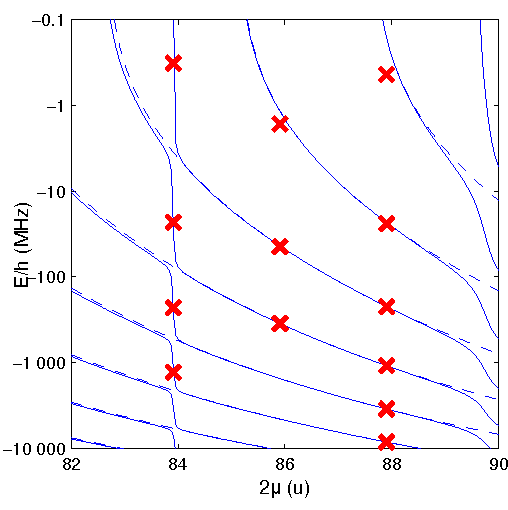
\includegraphics[width=0.7\linewidth]{Chapitres/Engineering highly entangled system of photoassociated 87Sr atoms/images/Figures_pour_theorie/mass_scaling.pdf}
\caption[fig:pa-mass-scaling]{This graph - extracted from \cite{borkowski_mass_2014}- confronts the experimental internal states in red crosses to their 
theoretical predictions for different reduced mass of strontium isotopes. The theoretical model guarantees approximated scales
for molecular lines of $^{87}Sr$ but not precisely because this model neglects the hyperfine interaction of the species.}
\label{fig:pa-mass-scaling}
\end{figure} 
In conclusion with this theoretical content combining these scaling laws with WKB and LeRoy-Bernstein models 
enable to predict the average positions of the vibrational states on the intercombination line. In the 
following section, we will demonstrate how these predictions are used to target the PA lines of $^{88}Sr$ 
and $^{87}Sr$ with the appropriate experimental parameters.

\section{Spectroscopy protocol and calibration of the PA laser}

\subsection{Gas preparation and isotope specificities}
I will now present our experiments consisting in identifying photoassociation lines of $^{87}Sr$ yet unexplored,
starting from a characterization of $^{88}Sr$ molecular lines abundantly published.\\
The photoassociation (PA) rate is strongly density-dependent, as detailed in Section 3.1.3. 
The experimental approach differs according to the quantum statistics of the isotope:
\begin{itemize}
    \item \textbf{Fermions ($^{87}$Sr):} High densities are achieved by optimizing evaporative cooling ramps once the atoms are loaded into the crossed Optical Dipole Trap (ODT).
    \item \textbf{Bosons ($^{88}$Sr):} The near-zero scattering length of $^{88}$Sr is detrimental to evaporative cooling, as it suppresses the elastic collisions necessary for thermalization. In this case, the final density relies almost exclusively on the efficiency of the preceding cooling and trapping stages (e.g., the MOT).
\end{itemize}

\hl{Once a dense cloud is obtained, the PA process is initiated by illuminating the atoms with a dedicated laser beam and all these datas are realised with a magnetic field of $B = 1.6 \pm$ mazimized for $\pi$ optical transitions.}

\subsection{Photoassociation lasers and their spectral characteristics}
\subsubsection{ECDL locking and frequency referencing}
The PA beam is primarily generated using an ECDL laser from MOGlabs brand: the association of a cateye system to an etalon settles the wavelength of the laser within a precision of $10^{-4}$ nm (architecture outlined in 1.3.2). 
One use a beating procedure to lock this laser: as detailed in figure \ref{frequences 88sr 87sr} the MOGLabs and "11/2 AOM" beams interfer on the same optical path intercepted by the "beating photodiode". The measured signal is 
then converted by the photodiode and mixed with an RF source to generate an error signal that is fed back to the MOGlabs laser current and piezo to stabilize the frequency. 

The optical path of the figure \ref{PA slave 1} shows a design of the "11/2" beam that is shared in a first arm for the optical pumping of the atoms and in a second one for the beating procedure. In the same place the beams from
repumper, MOGlabs and slave 1 are sent nearby to a wavemeter that is measuring one by one thanks to mechanical shutters.

\begin{figure}[H]
    \centering
    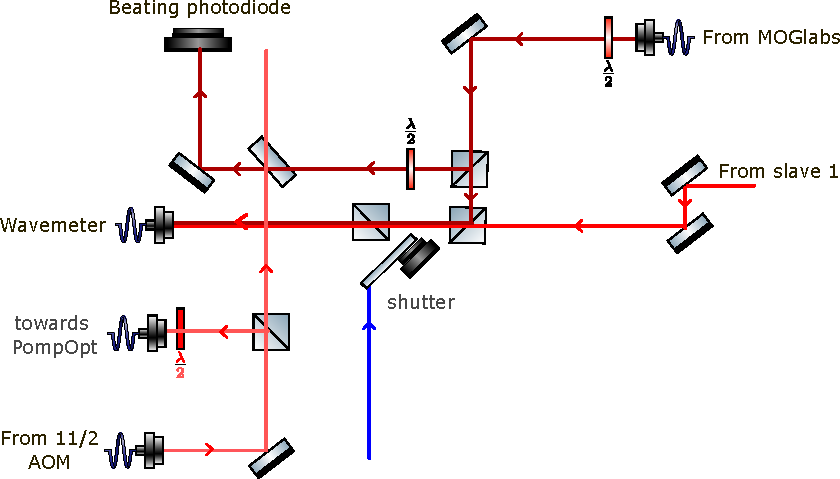
\includegraphics[width=1\linewidth]{Chapitres/Engineering highly entangled system of photoassociated 87Sr atoms/images/Schemas_optiques/nouveau_beating.pdf}
    \caption[PA slave 1]{Beating scheme for PA process between the light from "AOM 11/2" and MOGlabs. The light is coming from \ref{zoom red chain battement}
    to split in two arms: optical pumping and PA. This last one serves for MOGlabs locking in a beating procedure where the beam is recombined by the 50/50 waveplate
    superposing with slave 1 beam.}
    \label{PA slave 1}
\end{figure}
The final frequency of the PA beam depends on multiple RF and optical frequencies:
\begin{itemize}
    \item $f_{Red~master}$ is the optical frequency of the head master ECDL laser 
    \item $f^{RF}_{beating}$ the frequency used for demodulating the beating between 11/2 beam and MOGlabs. This RF source gives the error signal necessary for the wavelength 
    setting and stabilization of the MOGlabs laser.
    \item $f^{RF}_{Raman}$ the frequency of the "Raman AOM" used to shift the frequency beam of the PA beam in very last position of the scheme, also used for the Raman transitions used in the Ramsey interferometry
    schemes of Chapter 2
    \item $f^{RF}_{slave 1}$ is the frequency of the "Slave 1" AOM that is ahead of the lines for the $^{87}Sr$ MOT and the "11/2 AOM" responsible for the optical pumping and the beating.
    The shift of the diffracted order enables to go from the isotope 88 to the 87 (see 3.3.1)
    \item  $f^{RF}_{11/2}$ is the frequency of the "11/2 AOM" used for optical pumping and beating.
\end{itemize}


The frequency of the beam sent to the atoms is then given by the following formula:
\begin{equation}
    f_{PA} = f_{MOGlabs} + f^{RF}_{beating} - f^{RF}_{Raman} \pm 2\times f^{RF}_{slave 1} - 2\times f^{RF}_{11/2}
\end{equation}


The locking upper limit of the MOGlabs laser does not allow to reach frequencies above $f^{RF}_{beating} = 500$ MHz. 
A possibility to adress deeper bound vibrational states is to modify the different accessible frequencies -considering their RF frequency limits-
and/or invert the diffracted order of the "Raman AOM" that allows to shift the PA beam to about $\pm 260$ MHz.


\begin{figure}[H]
    \centering
    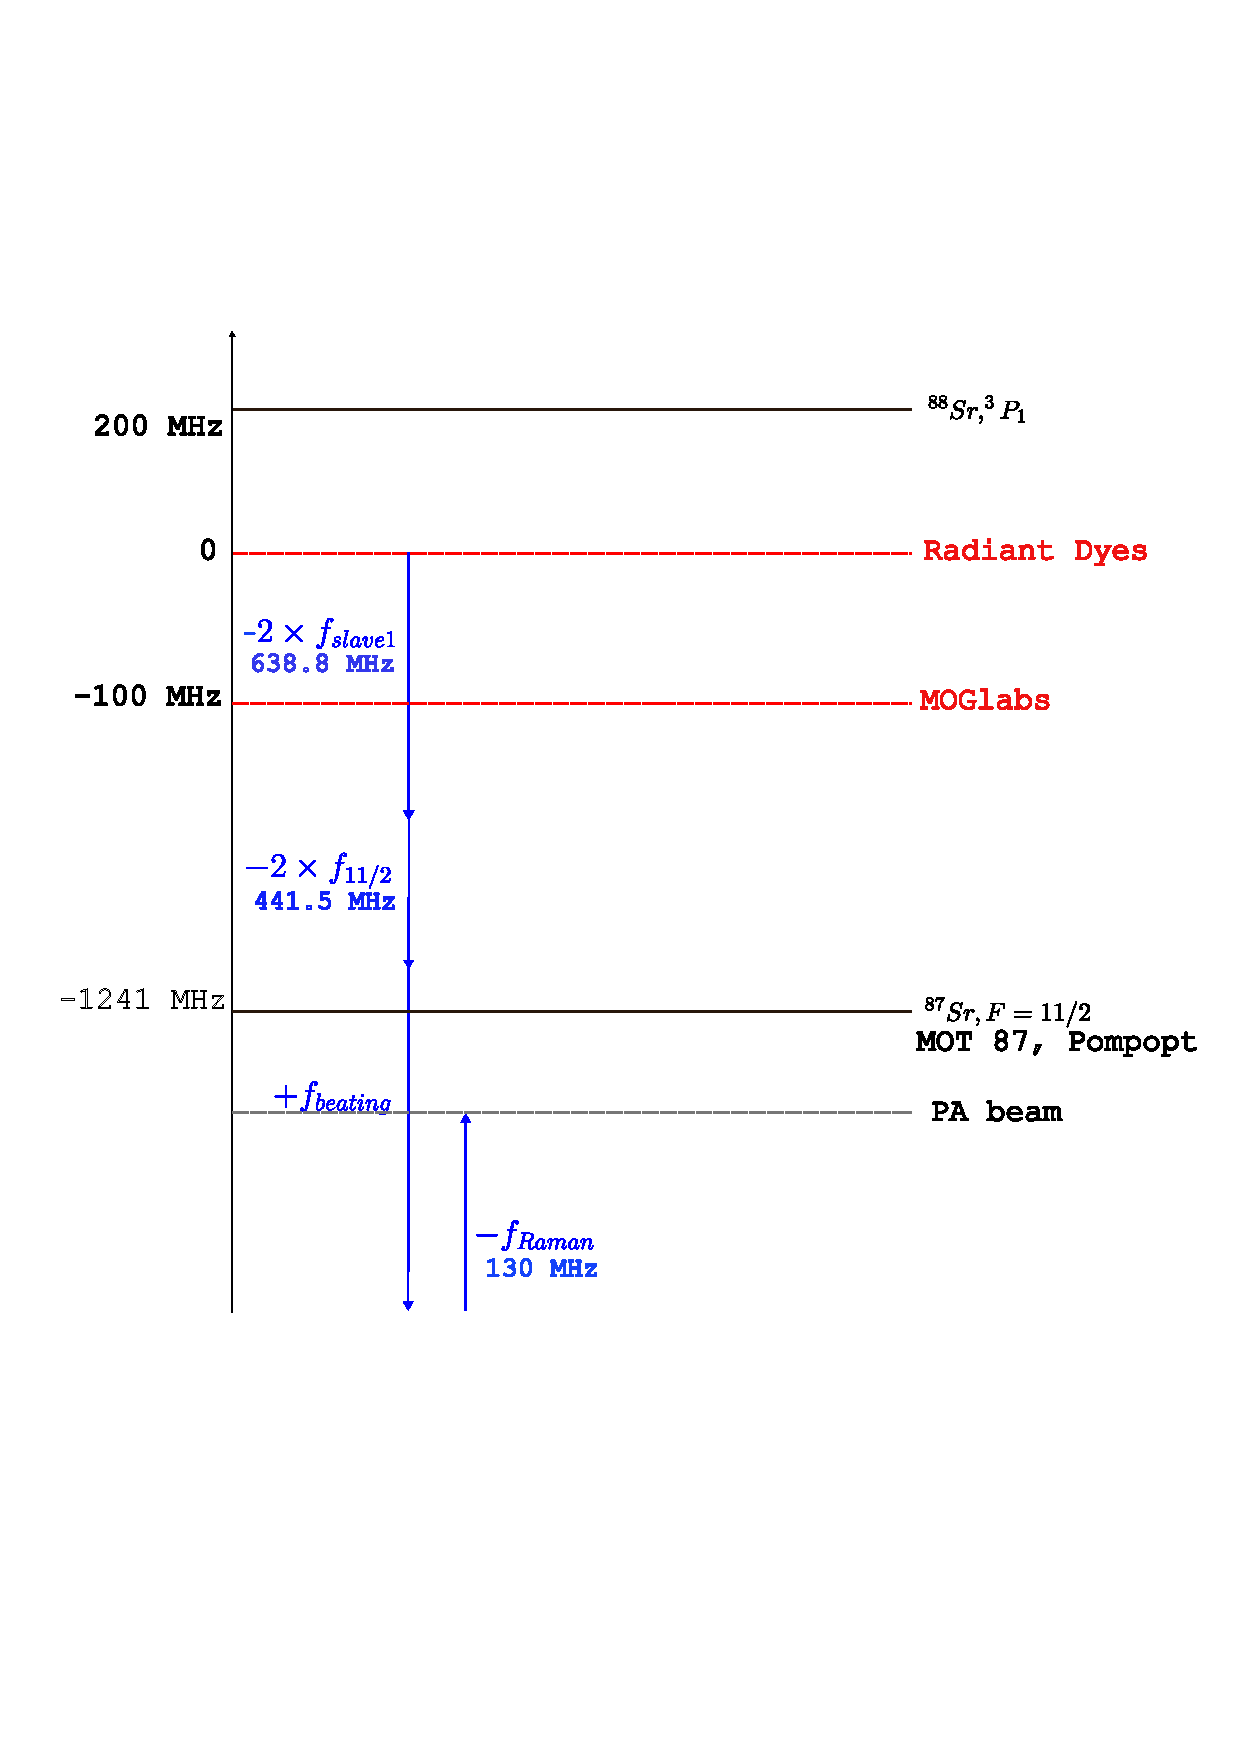
\includegraphics[width=0.8\linewidth]{Chapitres/Engineering highly entangled system of photoassociated 87Sr atoms/images/frequences_PA_87.pdf}
    \par\medskip
    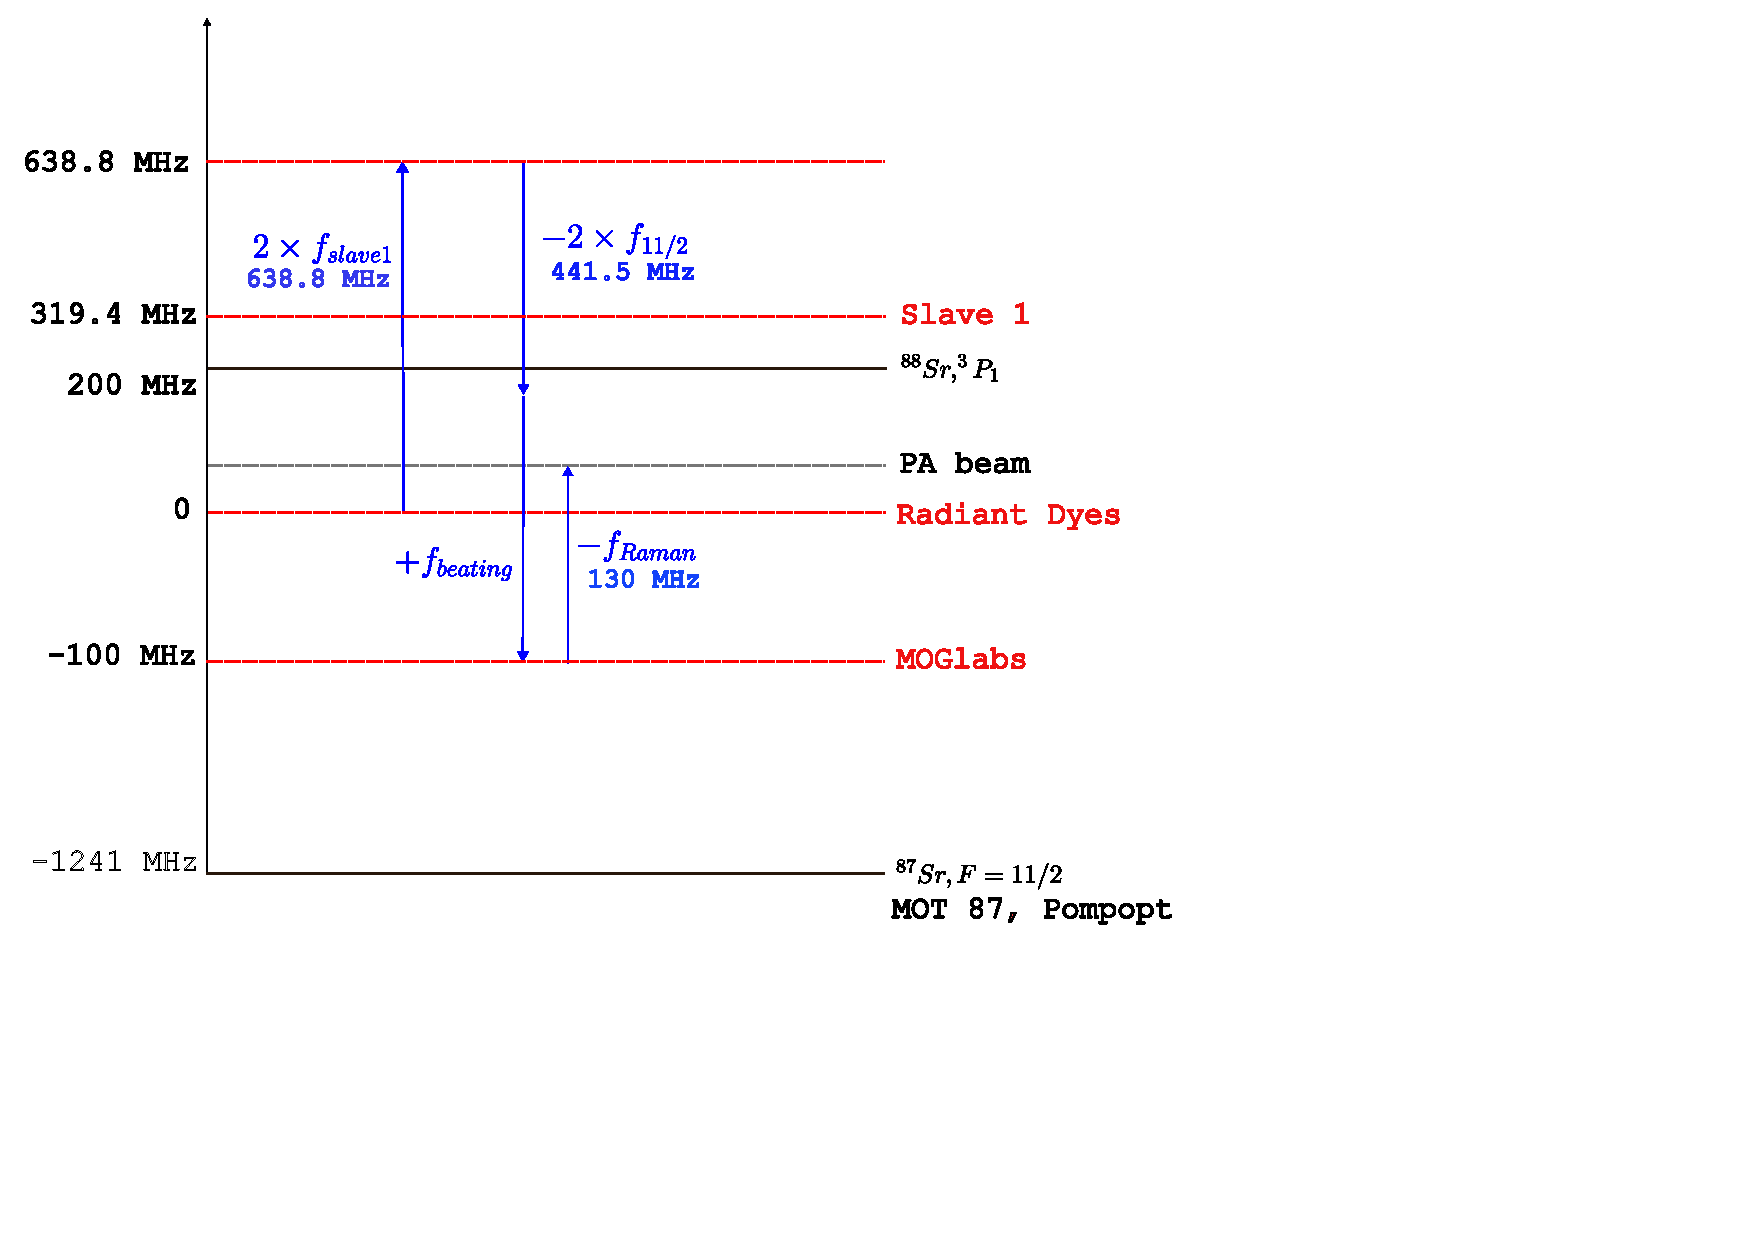
\includegraphics[width=0.85\linewidth]{Chapitres/Engineering highly entangled system of photoassociated 87Sr atoms/images/frequences_PA_88.pdf}
    \caption[frequences 88sr 87sr]{Frequency schemes for photoassociation (PA) depending on the targeted isotope: (top) scheme for $^{87}\text{Sr}$ and (bottom) scheme for $^{88}\text{Sr}$. 
    Switching the diffracted order of 'AOM Slave 1' allows for a seamless transition between isotopes, requiring only a minor realignment of the beam injection downstream of the AOM.}
    \label{frequences 88sr 87sr}
\end{figure}


\subsubsection{Spectral imperfections from the locking scheme}
The beating spectrum of the PA laser locking is presented in figure \ref{beating broadening} at a resonant bandwith RBW = 10kHz associated to a chosen video bandwith 
VBW = 300Hz. Expecting the molecular lifetime of $^{87}Sr$ to be $\Gamma_{mol} \simeq 15$ kHz this signal simulates the spectrum seen by the molecules.
Side components around $\pm 50$ kHz carry nearly half the measured electrical power of the beating signal: then only half the measured optical power is 
adressing the particules at the beating center frequency. 
This observation limits the power at which one can photoassociate the atoms. While the laser width is fine (\hl{~1kHz}) it also means that the linewidth of the molecule or the atoms - depending on 
the frequency of the PA laser- is broaden by the beating spectrum with side components.

\begin{figure}[H]
    \centering
    
\includegraphics[width=0.9\linewidth]{Chapitres/Engineering highly entangled system of photoassociated 87Sr atoms/images/Figures_pour_theorie/battement.pdf}
    \caption[Beating spectrum]{Beating spectrum between the MOGlabs laser and the "AOM 11/2" measured at the spectrum analyzer at RBW = 10 kHz and 
    VBW = 300 Hz. The side components at around $\pm 50$ kHz induce a broadening of the natural linewidth of atoms/molecules adressed by the PA beam
    coming from the MOGlabs head beat locked.}
    \label{beating broadening}
\end{figure}

\subsubsection{Spectral imperfections from the filter cavity system}
The laser passes through a Fabry-Perot cavity (see section 1.3.2) stabilized by a Pound-Drever-Hall (PDH) locking system containing an EOM. This latter modulates 
the incident electric field of frequency $f_0$ fixed at $f_M=40.48$ MHz (see \cite{black_Gas_preparation_and_spin_control_2001}). The phase modulation gives rise to interferences between the carrier at central frequency 
$f_0$ and the modulating signal at $f_M$:

\begin{equation}
    E_{inc}^{mod} = E_0 \left(J_0(\beta)e^{if_0t}+J_1(\beta)e^{i(f_0 + f_M)t}-J_1(\beta)e^{i(f_0-f_M)t}\right)
\end{equation}

The first term at amplitude $J_0(\beta)$ - the $0^{th}$ order Bessel function - is the incident electric field at frequency $f_0$ with effective amplitude $E_0 J_0(\beta)$. 
The second and third terms come from the interference of the carrier with the RF signal giving rise to two sidebands at $f_0\pm f_M$ with amplitude $J_1(\beta)$ the first order Bessel function.
Figure \ref{Bessel function} shows the ratio between the carrier and sidebands depending on the settled $\beta$.
Experimentally the modulation depth $\beta=1$ gives around five times more intensity in the carrier relative to the sidebands which is convenient to these constraints and directly tunable by the amplitude 
of the RF signal. 

\begin{figure}[H]
    \centering
    
\includegraphics[width=0.7\linewidth]{Chapitres/Engineering highly entangled system of photoassociated 87Sr atoms/images/Figures_pour_theorie/bessel_functions_finale.pdf}
    \caption[Bessel functions]{Modulus square of the $0^{th}$ and $1^{st}$ Bessel functions $J_n$ governing the power distribution between the carrier and PDH sidebands.}
    \label{Bessel function}
\end{figure}


We measured the effect of these sidebands on $500.000$ atoms gas evaporated and recompressed to a temperature $T = 4.1\mu K$. It is tested on the two spin components $m_f=-9/2, +9/2$ 
optically pumped during $2$ sec at optical power $I = 385$mW/cm$^2$ with the ECDL laser.
Plot \ref{fig:raie-40mhz} shows the number of atoms adressed by the positive sideband:
as schematized in \ref{sidebands} the presence of the sidebands triggers "ghost" resonances when the carrier is detuned by $f_0' = f_0 \pm f_M = f_0 \pm 40.48$ MHz 
from the atomic transition, leading to spurious one-body losses. The interfering components are also displaced by the same frequency.
Then the sideband at $f_0'-f_M$ visible in the purple signal is adressing the atomic transition at $f_0$ with a reduced amplitude comparing to the dark signal
previously centered in $f_0$.

\begin{figure}[H]
    \centering
        
\includegraphics[width=0.8\linewidth]{Chapitres/Engineering highly entangled system of photoassociated 87Sr atoms/images/Figures_pour_theorie/erreur_40MHz.pdf}
        \captionof{figure}{Scheme of the PDH sidebands addressing the atomic resonance. The purple plot is the dark signal -with the three interfering components
        between the carrier and the first harmonics- shifted by $f_0'-f_0$.}
        \label{sidebands}
\end{figure}

\begin{figure}[H]
    \centering
        
\includegraphics[width=1\linewidth]{Chapitres/Engineering highly entangled system of photoassociated 87Sr atoms/images/40MHz_resonance.pdf}
        \captionof{figure}{Atomic loss due to FP cavity PDH sideband that is adressing the $^1S_0 - ^3P_1$ line at $\Delta = f_0 - f_M$ with $f_M$ the 
        modulation frequency of the PDH EOM.}
        \label{fig:raie-40mhz}
\end{figure}

The double-peak shape of this resonance comes from the recovering of the ten different $m_F$ state that are populated by the PA laser imperfectly
polarized: a small purcentage of $\sigma$ polarization induces transitions to neighboring $m_F$ states. Measurement of the same data for different magnetic 
field values confirmed this hypothesis since the splitting evolved with. 

Settling lower modulation depth $\beta$ decreased the absolute amplitude of this curve but it was not possible to completly cancel this effect: molecular line
with small amplitude could be hiden in this signal.


\subsection*{Conclusion: Validation of the PA spectroscopic protocol}

The purpose of this section was to establish and validate the operational procedure to tune the PA laser frequency. Characterization of the laser system 
highlighted two critical experimental insights:
\begin{itemize}
    \item \textbf{Power calibration and spectral distribution:} Analyzing the beat-note signal revealed that approximately half 
    of the total laser power is distributed into unwanted frequency components. This spectral dilution directly contributes to the observed broadening of both 
    atomic and molecular spectroscopic lines.
    
    \item \textbf{Modulation-induced parasitic resonances:} Laser modulation can generate sidebands that induce unexpected atomic or molecular transitions. 
    Specifically, sidebands at $f_M = \pm 40.48$~MHz from the main line can lead to a misinterpretation of atom loss signals. In our setup, this modulation 
    originates from the electro-optic modulator (EOM) used for the Pound-Drever-Hall (PDH) lock, although similar effects can arise in the presence of 
    an optical device that can be modulated by an close RF source frequency such as acousto-optic modulators (AOMs).
\end{itemize}

\subsection{Atomic and molecular lines calibration}
\subsubsection{General experimental framework and baseline parameters}
In this section the PA experiments on $^{88}\text{Sr}$ begins with an initial density of $n_0 = 5 \times 10^{13}\text{ atoms/cm}^3$ and a temperature of $T \simeq 1.7\text{ }\mu\text{K}$. 
The atomic transition is addressed at $f^{\text{RF}}_{\text{beating}} = f_{\text{Raman}}$ using a laser beam with an intensity of $I = 100~I_{\text{sat}}$ and a waist of $w_0 = 340~\mu\text{m}$. 
The expected characteristic timescale for the illumination is defined by isolating the two-body loss term of Eq. \ref{one and two body losses equation}:
\begin{gather*}
    \frac{dn(t)}{dt} = -\beta n(t)^2 \\
    \int_{n_0}^{n(t)} \frac{dn}{n^2} = -\beta \int_{0}^{t} dt \\
    \left[ -\frac{1}{n} \right]_{n_0}^{n(t)} = -\beta t \\
    \frac{1}{n(t)} - \frac{1}{n_0} = \beta t \\
    t = \frac{1}{\beta} \frac{n_0 - n(t)}{n(t) n_0}
\end{gather*}

At half the initial density, the characteristic loss time $\tau$ is given by:
\begin{equation}
    \tau = \frac{1}{\beta n_0}
\end{equation}

Most of the spectroscopic lines presented below exhibit a two-body loss rate coefficient in the range of $10^{-12} < K_2 < 10^{-8}\text{ cm}^3\cdot\text{s}^{-1}$, implying that $\tau$ should typically be on the order of a few milliseconds or less. However, due to an unexpectedly low atom loss at resonance, it was subsequently determined that a spatial misalignment of the PA beam relative to the atomic cloud induced a significant spatial inhomogeneity. Consequently, all the data presented for $^{88}\text{Sr}$ were obtained with a prolonged illumination time of approximately $800\text{ ms}$.

Furthermore at resonance an illumination time of $800\text{ ms}$ with saturating intensity corresponds a scattering rate $\Gamma_{at}/2$. Then the number of scattered photons is $N = \Gamma_{at}/2 \times t \simeq 10^4$ scattered photons per atom. This induces severe heating of the atomic cloud, leading to a significant thermal broadening of the molecular resonances.

The bottom panel of fig.\ref{frequences 88sr 87sr} displays the atom loss at this reference frequency.
Then the laser MOGlabs robustly locked, we change $f^{RF}_{beating}$ to search the three first vibrational states visible in figure
\ref{88Sr resonance}. 

\subsubsection{Fitting model}
I deduced the number of atoms plotted in the following figures from the two-dimensional integration of the optical density, following the method demonstrated in Ref.~\cite{litvinov_measuring_2021}. 
Each data point of the presented atomic and molecular lines is extracted by fitting the absorption images of the atomic cloud with a 2D Gaussian function. The fit covariance yields a relative fitting uncertainty defined as:

\begin{equation}
    \sigma_{\text{gaussian}} = \sqrt{\left(\frac{\delta A}{A}\right)^2 + \left(\frac{\delta \sigma_x}{\sigma_x}\right)^2 + \left(\frac{\delta \sigma_y}{\sigma_y}\right)^2}
\end{equation}

where $\delta A$, $\delta \sigma_x$, and $\delta \sigma_y$ are the diagonal elements of the fit covariance matrix, corresponding respectively to the amplitude and the spatial widths along the $x$ and $y$ axes.

When sweeping the laser frequency across an atomic or molecular resonance, the evolution of the atom number exhibits a Lorentzian profile:

\begin{equation}
    f(x) = y_0 + \frac{A}{(x-x_0)^2 + \left(\frac{\Gamma}{2}\right)^2}
\end{equation}

characterized by a full-width at half-maximum (FWHM) $\Gamma$, centered at $x_0$, with a peak amplitude $A / (\Gamma/2)^2$ and an offset $y_0$.

To account for shot-to-shot experimental fluctuations, the RMS atom number variation over ten consecutive realizations was included. The total uncertainty associated with each atom number measurement is given by:

\begin{equation}
    \sigma_N^{\text{tot}} = N \sqrt{\sigma_{\text{gaussian}}^2 + \sigma_{\text{systematic}}^2}
\end{equation}

The resonances exhibit an effective linewidth $\Gamma_{\text{tot}}$ resulting from physical and technical broadening mechanisms:

\begin{equation}
    \Gamma_{\text{tot}} = \sqrt{\Gamma_0^2 + \Gamma_{\text{thermal}}^2 + \Gamma_{\text{laser}}^2 + \Gamma_{\text{remainder}}^2}
\end{equation}

where $\Gamma_0$ is the natural linewidth ($\Gamma_0 = 2\pi \times 7.5\text{ kHz}$ for the $^1S_0 - ^3P_1$ atomic line of $^{88}\text{Sr}$, and $\Gamma_0 \approx 15\text{ kHz}$ on average for the molecular states). Due to small Franck-Condon factors, the effective saturation intensity $I_{\text{sat}}^{\text{eff}}$ for molecular transitions is significantly larger than for atomic ones, making power broadening completely negligible for molecular lines \cite{zelevinsky_narrow_2006}.

Furthermore, the thermal motion of Doppler-shifted atoms introduces a thermal broadening given by:

\begin{equation}
    \Gamma_{\text{thermal}} = \frac{1}{\lambda}\sqrt{\frac{k_B T}{\mu}} 
\end{equation}

with $\mu = m_{\text{at}}/2$ for molecular resonances, $\mu = m_{\text{at}}$ for single atoms, $\lambda$ the laser wavelength, $T$ the gas temperature, and $k_B$ the Boltzmann constant. 

Finally, $\Gamma_{\text{laser}}$ accounts for the intrinsic spectral width of the laser source, while $\Gamma_{\text{remainder}}$ gathers unassigned technical broadening sources. By subtracting the known physical contributions ($\Gamma_0, \Gamma_{\text{thermal}}$) in quadrature from the measured total linewidth $\Gamma_{\text{tot}}$, one can isolate the effective technical laser linewidth:

\begin{equation}
    \Gamma_{\text{laser+rem}} = \sqrt{\Gamma_{\text{tot}}^2 - \left(\Gamma_0^2 + \Gamma_{\text{thermal}}^2\right)}
\end{equation}


\subsubsection{Experimental results on $^{88}$Sr}
The first molecular state shown in the middle panel of Fig.~\ref{88Sr resonance} was detected using an exposure time of $t = 1000$~ms and an intensity of $I = 826$~mW/cm$^2$. This state is located at a detuning of $f = -23.99 \pm 0.01$~MHz from the atomic transition (measured with the MOGlabs laser system), revealing a total effective linewidth of $\Gamma_{\text{tot}} = 192 \pm 9\text{ kHz}$. Accounting for the natural width $\Gamma_0 = 15\text{ kHz}$ and a thermal broadening estimated at $\Gamma_{\text{thermal}} = 19\text{ kHz}$, the residual technical broadening is deduced to be $\Gamma_{\text{laser+rem}} = 190.47\text{ kHz}$\hl{$\pm$}.

Subsequently, a second resonance was observed using the same laser system at a detuning of $f = -222.70 \pm 0.01$~MHz, with a beam intensity of $I = 303$~mW/cm$^2$ and an exposure time of $50$~ms. The measured linewidth of this second resonance was $\Gamma_{\text{tot}} = 330 \pm 13\text{ kHz}$, with a thermal broadening contribution of $\Gamma_{\text{thermal}} = 21\text{ kHz}$. Subtracting these physical terms yields a technical laser width of $\Gamma_{\text{laser+rem}} = 328.99\text{ kHz}$\hl{$\pm$}.

These experimental findings agree well with the results reported by Zelevinsky et al.~\cite{zelevinsky_narrow_2006}, who identified vibrational states at $f_{\nu=-1} = -23.932(33)$~MHz and $f_{\nu=-2} = -222.161(35)$~MHz associated with the $0_u$ photoassociation potential. 
The tensorial light shift induced by the photoassociation (PA) beam causes a frequency shift in these molecular states, as investigated by Blatt et al.~\cite{blatt_measurement_2011}, where the $\nu = -2$ state exhibited a red-shift of $200$~kHz for a laser intensity increase of approximately $800$~mW/cm$^2$.

The measured linewidths ($\Gamma_{\text{tot}} \sim 192\text{--}330\text{ kHz}$) remain significantly larger than the expected intrinsic molecular linewidth of $\Gamma_0 \approx 15\text{ kHz}$. This substantial broadening stems from technical limitations, notably laser phase noise and sidebands (see section 3.2.2.2). To confirm that this broadening was technical, we measured the same molecular line with an alternative, higher-stability laser source.

\begin{figure}[htbp]
    \centering
    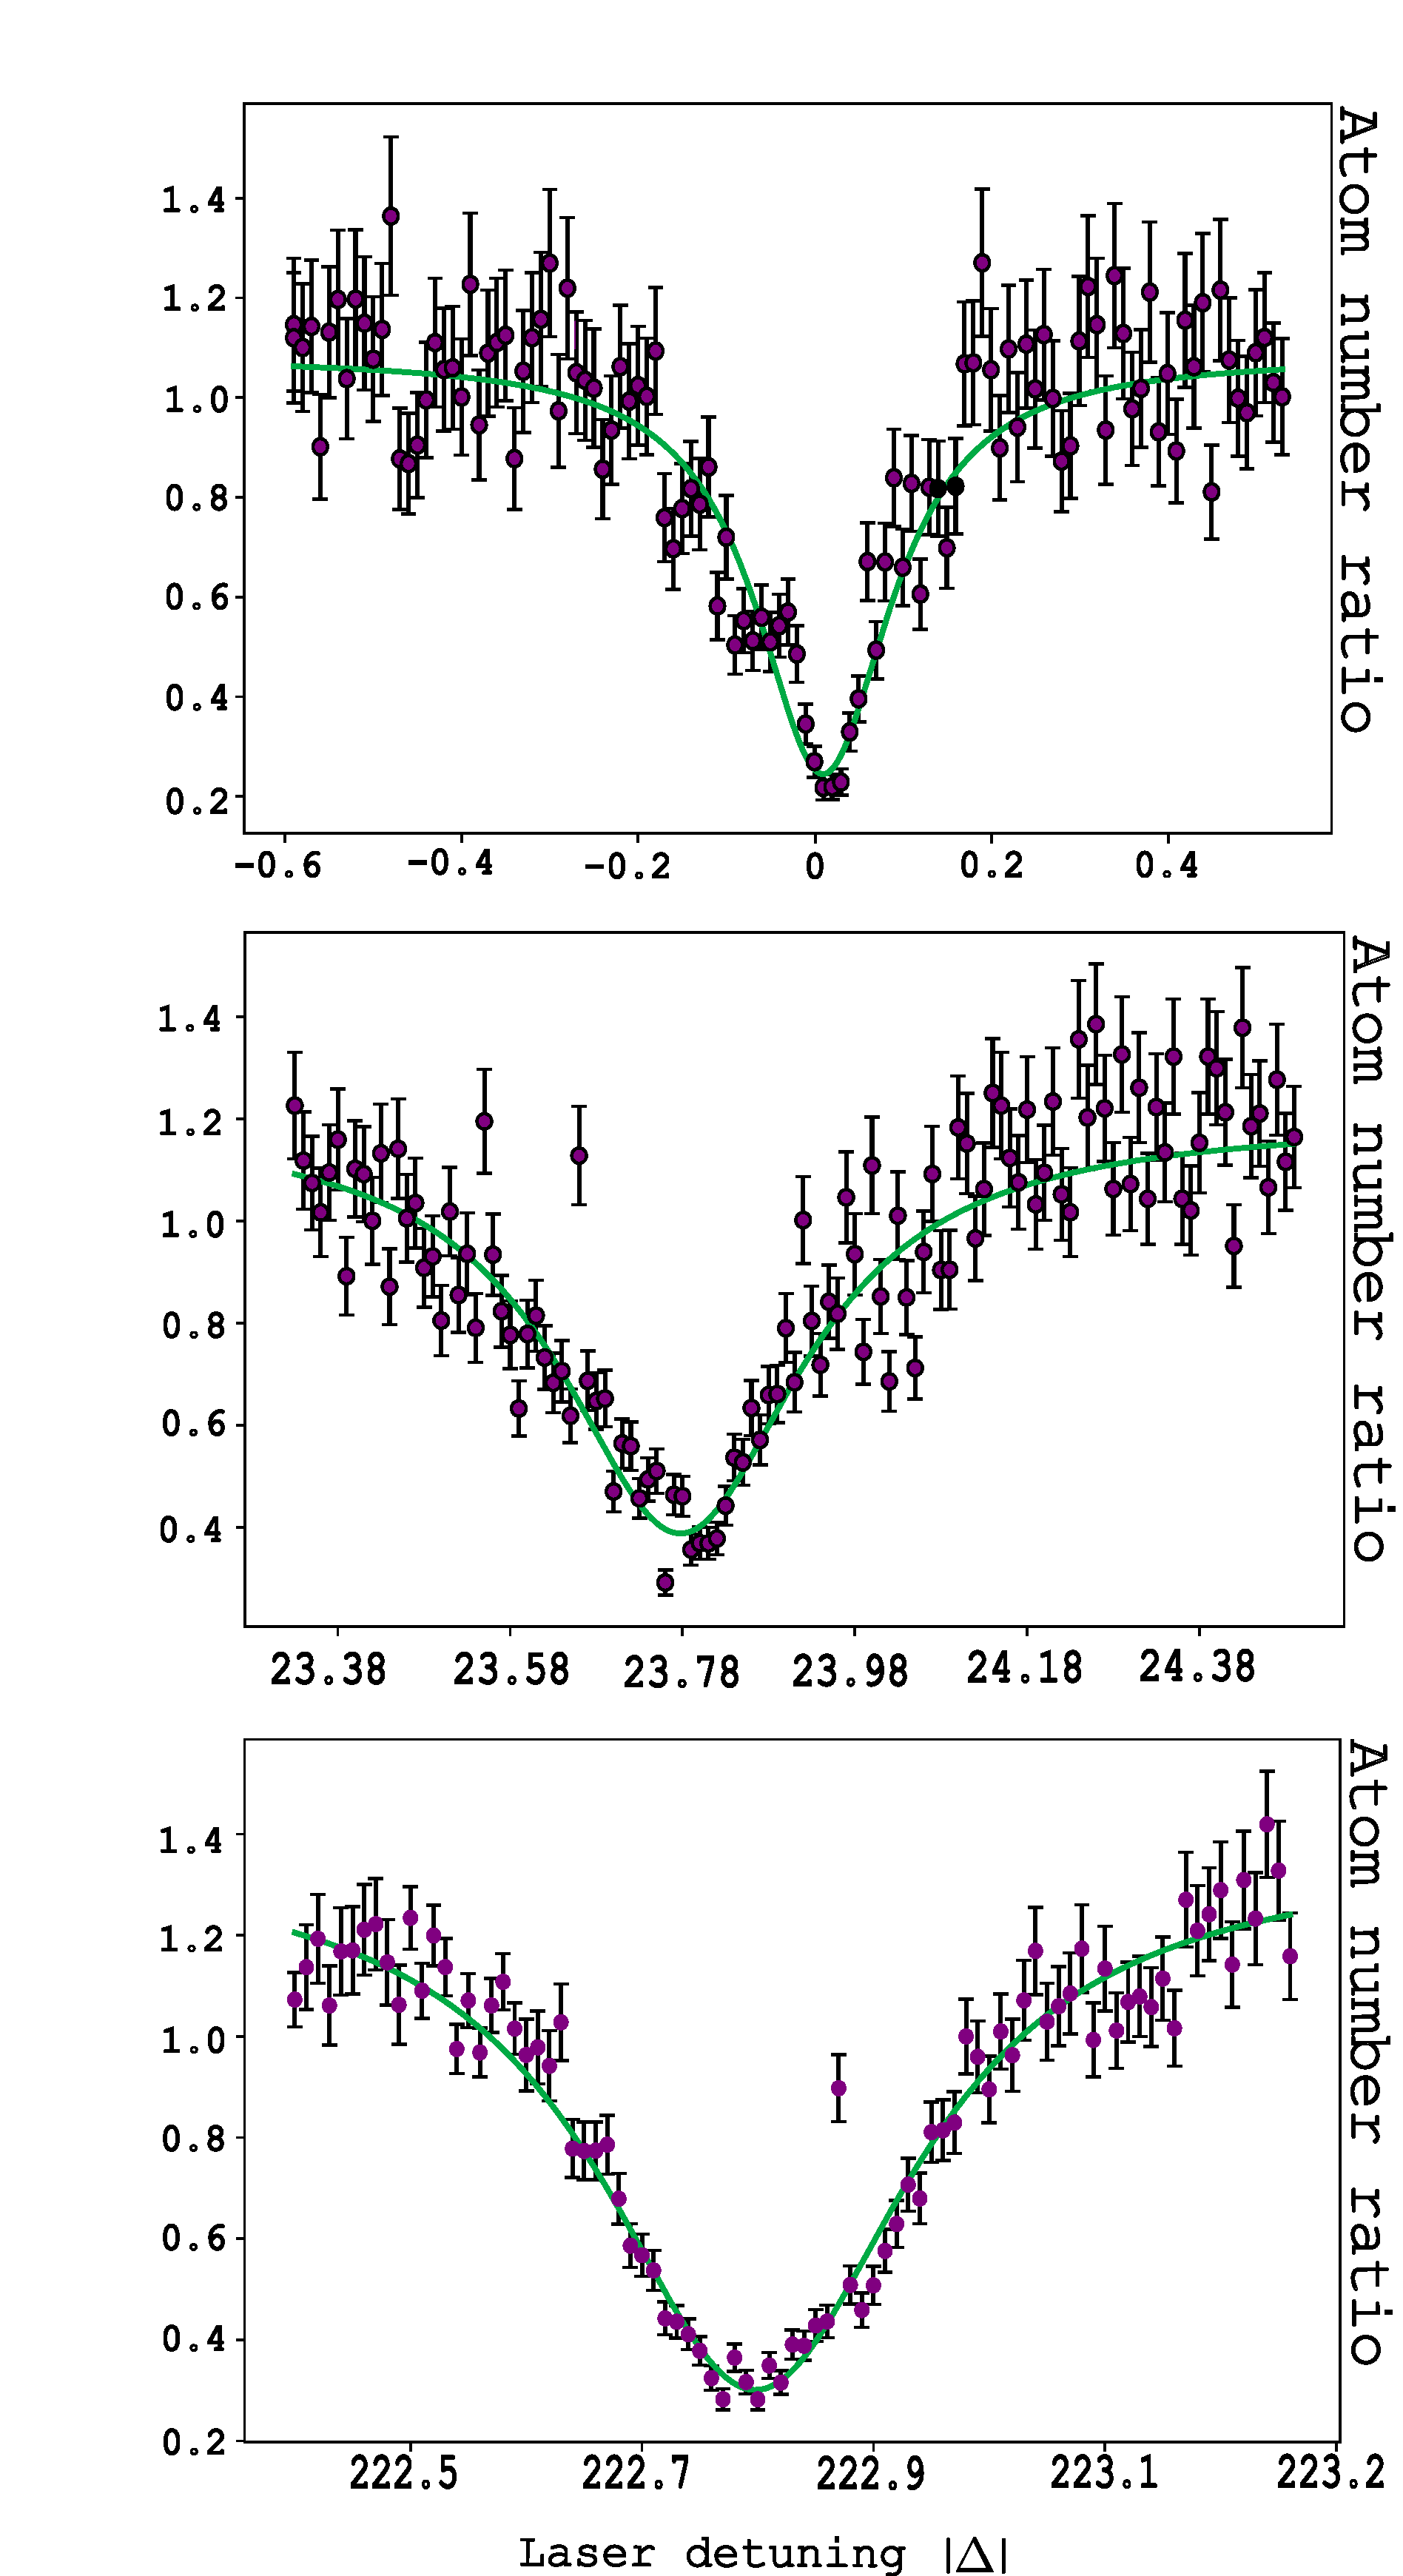
\includegraphics[width=0.75\linewidth]{Chapitres/Engineering highly entangled system of photoassociated 87Sr atoms/images/88Sr/resonance_88.pdf}
    \caption[Resonances of $^{88}\text{Sr}$]{Normalized $^{88}\text{Sr}$ atom number across the intercombination line. 
    (Top) Atomic resonance used as the PA frequency reference. Data points are extracted from 2D Gaussian fits of absorption images; error bars include fit covariance and unperturbed cloud RMS fluctuations. 
    (Middle) $\nu = -1$ vibrational state ($I = 826$~mW/cm$^2$, $1000$~ms). 
    (Bottom) $\nu = -2$ vibrational state ($I = 303$~mW/cm$^2$, $50$~ms). 
    Solid lines are Lorentzian fits with errors accounting for covariance and systematic fluctuations.}
    \label{88Sr resonance}
\end{figure}


\subsubsection{Alternative source: the injection-locked laser}
Spectroscopy measurements confirmed the significant broadening induced by the MOGlabs ECDL laser. To demonstrate its technical origin, we compared the MOGlabs results with a more stable laser source: the "11/2 AOM" beam. The measured parameters for the $\nu = -2$ molecular state are summarized in Table~\ref{tab:comparaison_lasers} and illustrated in Figure~\ref{linewidth avec pompopt}.

\begin{table}[ht]
\centering
\caption{Experimental comparison of the $\nu=-2$ molecular resonance linewidth measured with two different laser sources.}
\label{tab:comparaison_lasers}
\begin{tabular}{|l|c|c|}
\hline
\textbf{Parameters} & \textbf{AOM 11/2 beam} & \textbf{MOGlabs laser} \\ \hline
Detuning $f$ [MHz] & $-222.70 \pm 0.01$ & $-222.70 \pm 0.01$ \\ \hline
Intensity $I$ [mW/cm$^2$] & $\mathbf{[VAL\_AOM]}$ & $303$ \\ \hline
Natural width $\Gamma_0$ [kHz] & $15$ & $15$ \\ \hline
$\Gamma_{\text{thermal}}$ (calc.) [kHz] & $21$ & $21$ \\ \hline
\textbf{Total measured width $\Gamma_{\text{tot}}$} [kHz] & $115.5 \pm 8.8$ & $344.5 \pm 27.3$ \\ \hline
\textbf{Deduced technical width $\Gamma_{\text{laser+rem}}$} [kHz] & $112.58$ & $328.99$ \\ \hline
\end{tabular}
\end{table}

\begin{figure}[H]
    \centering
    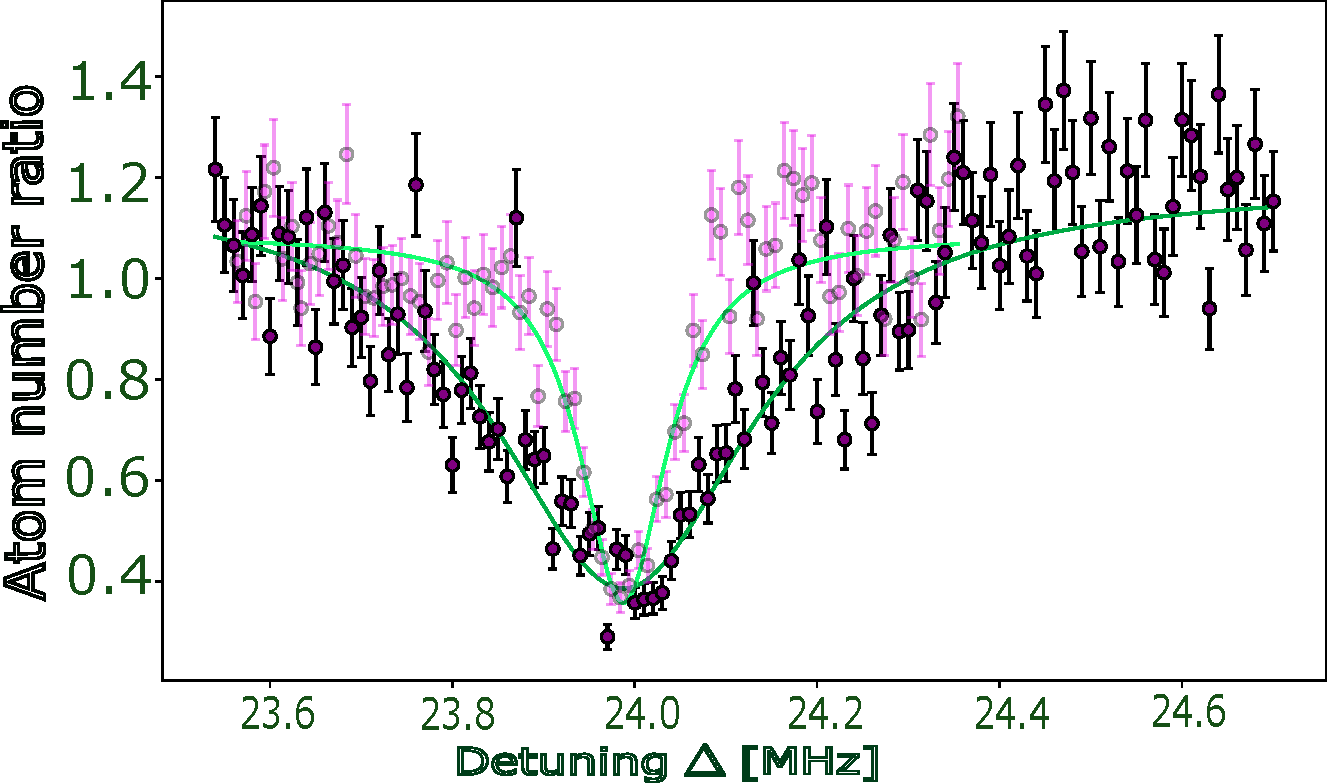
\includegraphics[width=1\linewidth]{Chapitres/Engineering highly entangled system of photoassociated 87Sr atoms/images/88Sr/comparaison_raie_24MHz_88_jolie.pdf}
    \caption[]{Comparison of the $\nu = -2$ molecular line profile. The MOGlabs dataset (deep purple) yields a line three times broader than the stable "11/2 AOM" source (light purple). MOGlabs frequencies were shifted for visualization clarity.}
    \label{linewidth avec pompopt}
\end{figure}

The MOGlabs source yields a technical linewidth $\Gamma_{\text{laser+rem}}$ approximately three times larger than the "11/2 AOM" beam. Nevertheless, the MOGlabs laser remains essential for broad spectroscopic searches due to its wide frequency tunability.

\subsubsection{Noise of the diode}
While comparing the broadening of the molecular line with two different lasers the spectroscopy revealed from the Thorlabs red diode \textbf{HL6750MG}, noise at $\pm 6$ MHz and $\pm 12$ MHz from the central frequency $f_0$. 
This effect has been observed on the $F = 9/2$ hyperfine state of $^{87}Sr$ that has twelve states of total spin projection $-11/2 < m_F < 11/2$ and that we were capable of resolving as visible in
\ref{6MHz noise red detuned}. The same measurement blue detuned from the atomic resonance confirmed in fig. \ref{6MHz noise blue detuned} the atomic nature of the losses. Starting from the atomic resonance 
at 0~MHz one decrease the frequency of the beating-note: centered in around -6~MHz and 
-12~MHz we see the presence of around twelve peaks that corresponds to the hyperfine state targeted.
\hl{mean temperature of the gas, SU(10)...}
Looking for molecular lines around +6~MHz and +12~MHz with the 11/2 beam is then compromised by the presence of these peaks.

\begin{figure}[H]
    \centering
    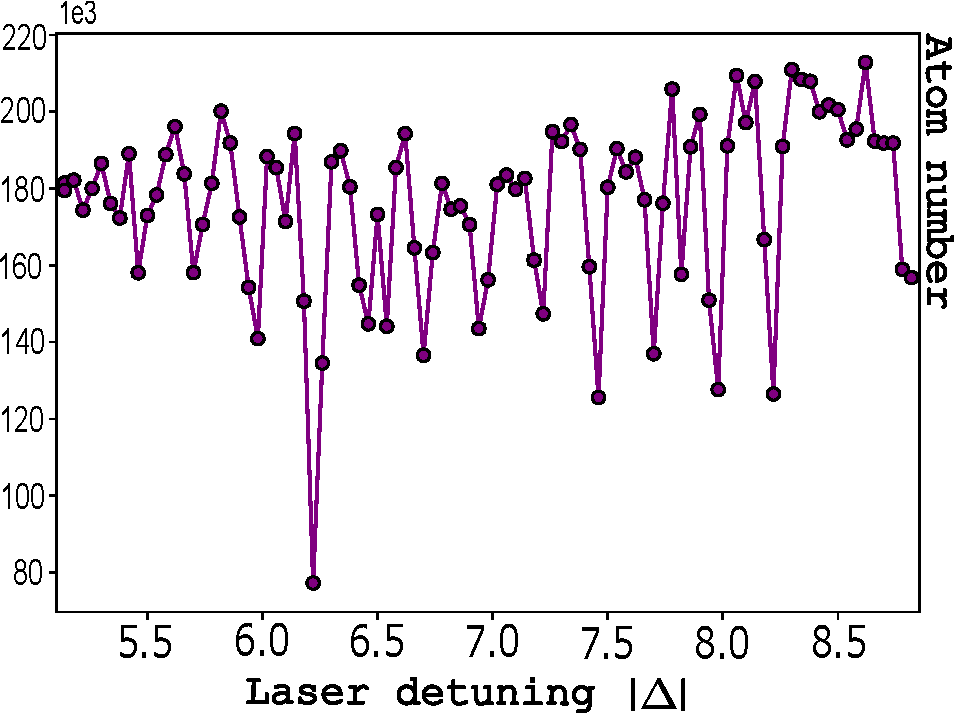
\includegraphics[width=0.8\linewidth]{Chapitres/Engineering highly entangled system of photoassociated 87Sr atoms/images/87Sr/data15_6MHz_noise.pdf}
    \caption[]{Twelve $m_F$ states of $F=11/2$ hyperfine state measured in an SU(10) gas at $\delta = +6~MHz$ from the atomic resonance. The presence of these peaks comes from a noise at this frequency coming 
    with the red diode. }
    \label{6MHz noise red detuned}
\end{figure}

\begin{figure}[H]
    \centering
    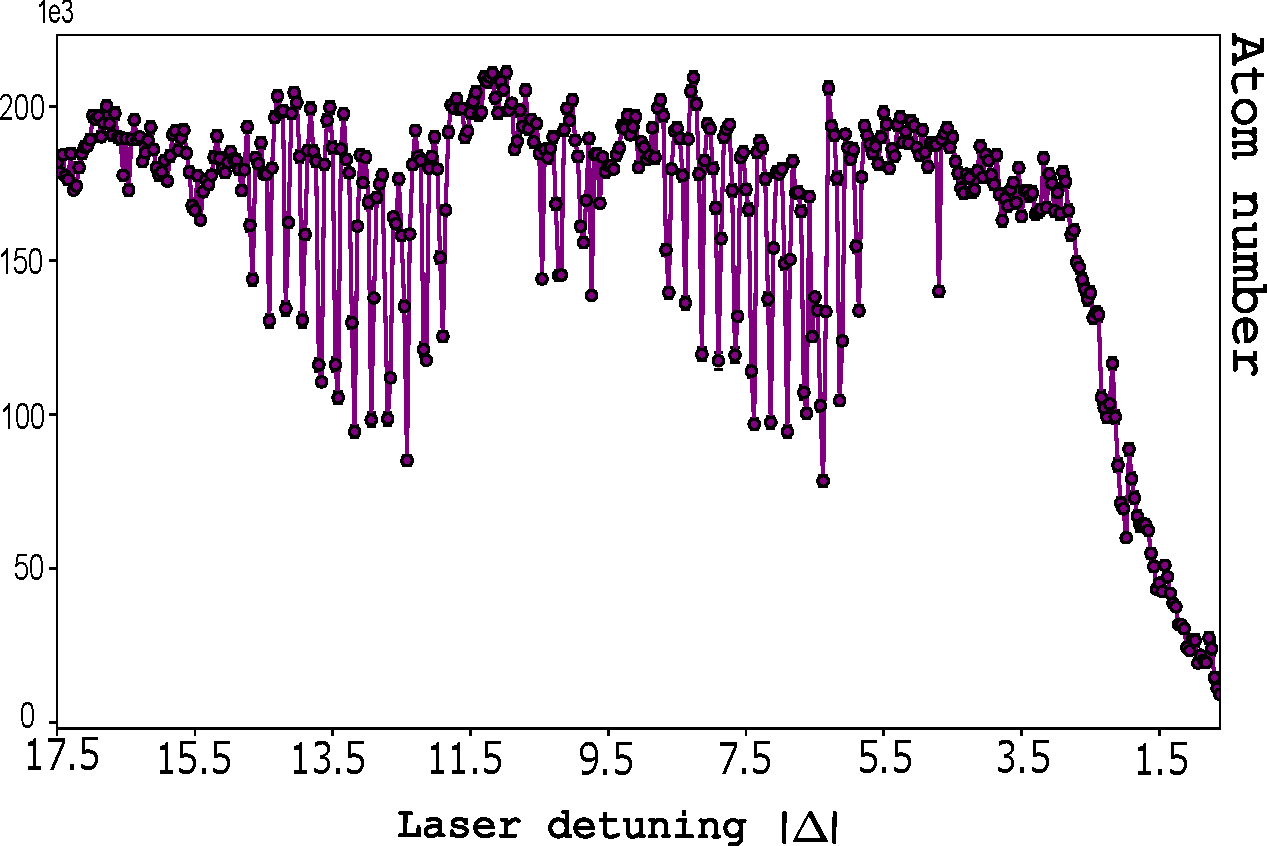
\includegraphics[width=0.8\linewidth]{Chapitres/Engineering highly entangled system of photoassociated 87Sr atoms/images/87Sr/6MHz_blue_detuned.pdf}
    \caption[]{Twelve $m_F$ states of $F=11/2$ hyperfine state measured in an SU(10) gas at $\delta = -6~MHz$ and $\delta = -12~MHz$ from the atomic resonance. 
    The presence of these peaks comes from a noise at this frequency coming 
    with the red diode.}
    \label{6MHz noise blue detuned}
\end{figure}

\subsubsection{Decay dynamics ($dN/dt$)}
The ultimate verification of inelastic nature of collisions is the time evolution of the atom number $dN/dt$ discussed in Section~3.1.3. This curve allows one to (i) verify the presence of two-body losses and (ii) 
determine the value of $l_{\text{opt}}/I$ which characterizes the strength of the loss rate $\beta$. The fitting function is obtained by integrating the rate equation:
\begin{gather}
    \frac{dN(t,T)}{dt} = -\beta(T(t)) N(t,T)^2 - \Gamma N(t,T) \label{eq globale collisions} \\[1.5ex]
    \text{Setting } M(t,T) = N(t,T)e^{\Gamma t} \iff N(t,T) = M(t,T)e^{-\Gamma t} \label{eq:change_var} \\[1.5ex]
    \dot{M}(t,T)e^{-\Gamma t} - \Gamma M(t,T) e^{-\Gamma t} = -\beta(T(t)) M(t,T)^2 e^{-2\Gamma t} - \Gamma M(t,T) e^{-\Gamma t} \label{eq:diff} \\[1.5ex]
    \int_{0}^{t} \frac{\dot{M}(t',T)}{M(t',T)^2} \, dt' = -\int_{0}^{t} \beta(T(t')) e^{-\Gamma t'} \, dt' \label{eq:integ} \\[1.5ex]
    -\frac{1}{M(t,T)} + \frac{1}{N_0} = -\int_{0}^{t} \beta(T(t')) e^{-\Gamma t'} \, dt' \label{eq:inv_M} \\[1.5ex]
    M(t,T) = \frac{N_0}{1 + N_0 \int_{0}^{t} \beta(T(t')) e^{-\Gamma t'} \, dt'} \label{eq:sol_M} \\[1.5ex]
    N(t,T) = \frac{N_0 e^{-\Gamma t}}{1 + N_0 \int_{0}^{t} \beta(T(t')) e^{-\Gamma t'} \, dt'} \label{eq:final_fit}
\end{gather}

Because $N(t,T)$ depends on the temperature, one wants to re-express Eq.~\ref{eq:final_fit} by explicitly showing the $T$-dependence of $\beta(T)$. The atoms are trapped in an ODT with a mean trapping frequency $\bar{\omega} = (\omega_x \omega_y \omega_z)^{1/3}$. According to the equipartition theorem, the spatial width $\sigma_{i}$ (with $i=\{x,y,z\}$) of the Gaussian distribution relates to the temperature $T$ via $\frac{1}{2}m_{\text{at}}\omega_{i}^2\sigma_{i}^2 = \frac{1}{2}k_B T$. This yields the effective volume:

\begin{equation}
    V_e(T) = (2\pi)^{3/2}\left(\frac{k_B T}{m_{\text{at}}}\right)^{3/2} \frac{1}{\omega_x\omega_y\omega_z} = (2\pi)^{3/2}\left(\frac{k_B T}{m_{\text{at}}\bar{\omega}^2}\right)^{3/2}
\end{equation}

with $\bar{\omega}=2\pi 50$~rad/s. By substituting $\beta(T(t')) = \frac{K_2}{2\sqrt{2}V_e(T(t'))}$ into the population evolution law, the final fitting equation becomes:

\begin{equation}
    N(t,T) = \frac{N_0 e^{-\Gamma t}}{1 + \left[ \frac{K_2}{8\pi^{3/2}} \left( m_{\text{at}} \right)^{3/2} \omega_x\omega_y\omega_z \right] N_0 \int_{0}^{t} \left( \frac{1}{k_B T(t')} \right)^{3/2} e^{-\Gamma t'} \, dt'}
\label{equation fit finale}
\end{equation}

This fitting function is used to extract the two-body loss rate coefficient $K_2$ from the experimental data. The temperature $T(t)$ is numerically interpolated from the measured temperature. Then for each illumination time, the integrale of \ref{equation fit finale} is calculated and the experimental data are fitted to extract $K_2$.\\

From equation \ref{eq globale collisions}, one expects two distinct slopes on the decay curve: an initial fast two-body decay regime followed by a slow one-body regime as the atomic density drops.\\ 

Figure~\ref{88sr exponential decay} illustrates these two regimes. The experimental data are adjusted using this model, from which the $\beta$ value is extracted. For the resonance $f_{\nu=2}=-222.161(35)$~MHz, the deduced optical length is $l_{\text{opt}} = 13 \, a_0/(\text{W/cm}^2)$, which can be compared to the value of $l_{\text{opt}} = 1 \, a_0/(\text{W/cm}^2)$ reported in \cite{zelevinsky_narrow_2006}. For the second line, we measure $l_{\text{opt}} = 7.6\times 10^3 \, a_0/(\text{W/cm}^2)$, which is consistent with the theoretical predictions from \cite{blatt_systematic_2011}.
\begin{figure}[H]
    \centering
    \begin{subfigure}[t]{0.48\linewidth}
        \centering
        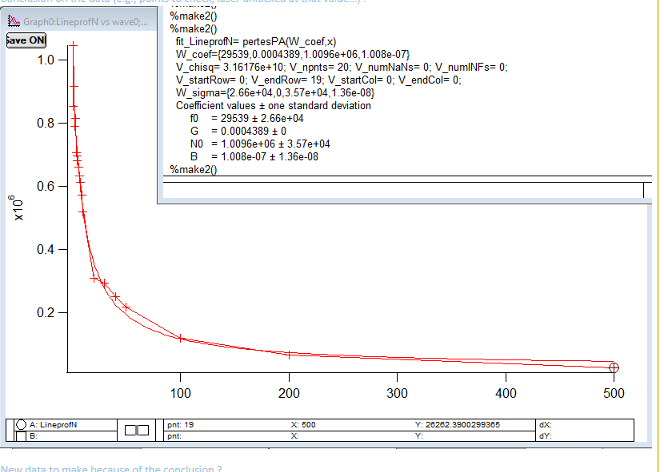
\includegraphics[width=1\linewidth]{Chapitres/Engineering highly entangled system of photoassociated 87Sr atoms/images/88Sr/data149_n2_88sr_moglabs.png}
    \end{subfigure}
    \hfill
    \begin{subfigure}[t]{0.48\linewidth}
        \centering
        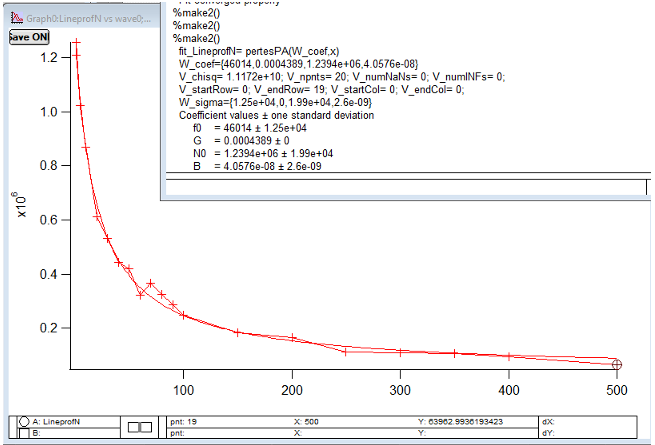
\includegraphics[width=1\linewidth]{Chapitres/Engineering highly entangled system of photoassociated 87Sr atoms/images/88Sr/data148_n3_88sr_moglabs.png}
    \end{subfigure}
    \caption[88sr exponential decay]{Needs to be replaced with data }
    \label{88sr exponential decay}
\end{figure}

The results obtained for the $^{88}\text{Sr}$ isotope are in good agreement with the literature. This calibration establishes a reliable baseline to search for $^{87}\text{Sr}$ molecular lines, provided the following experimental constraints are taken into account:
\begin{itemize}
    \item \textbf{Parasitic RF sidebands:} Measurements performed with the 11/2 AOM beam exhibit noise components at $\pm$6~MHz and $\pm$12~MHz, which can drive parasitic transitions apart from the main carrier frequency.
    
    \item \textbf{Laser-induced broadening:} The MOGlabs laser broadens the molecular lines slightly more than the 11/2 beam, though this contribution remains minor.
    
    \item \textbf{Thermal and power effects:} Driving the PA transition at high intensity significantly heats the gas, resulting in substantial thermal broadening of the spectroscopic lines. While power broadening primarily affects the atomic reference line, an additional, yet unidentified, broadening mechanism persists.
    
    \item \textbf{Loss dynamics:} At a variable (or stable) temperature, the time evolution of the atom number is accurately described by Eq.~\ref{eq:final_fit}, derived from the integration of the combined one- and two-body loss equation: $\frac{dN}{dt} = -\beta N^2 - \Gamma N$.
\end{itemize}

\section{$^{87}\text{Sr}$ molecules}

\subsection{Results on $^{87}Sr$}
The molecular lines on $^{87}Sr$ have been reached only with the MOGlabs source. To adress the fermionic species I did change the diffracted order of the red optical chain for the opposite order to adress $F=11/2$ hyperfine state $1.441$~GHz from the bosonic species 88. 
(see Setup \ref{zoom red chain battement}). \\
Datas have been obtained for different waist size in an effort to increase two-body losses, same for the density of the cloud. \\
For this species with hyperfine structure one expect to visualize hundreds of states as described in the theoretical part of this section
each wide of about 15~kHz.\\

All the resonances presented in this section are done with a shot-to-shot normalisation method in order to suppress short time derivation due to experimental 
fluctuation. The first atomic number measured during the experiment is the measurement of the atomic density in absence of the PA laser. The second one is the
measurement of the effect of the PA laser in the gas. This is repeated for the entire experiment and the final plots are the ratio of the perturbated gas on the 
non-perturbated one.

\begin{figure}[H]
    \centering
    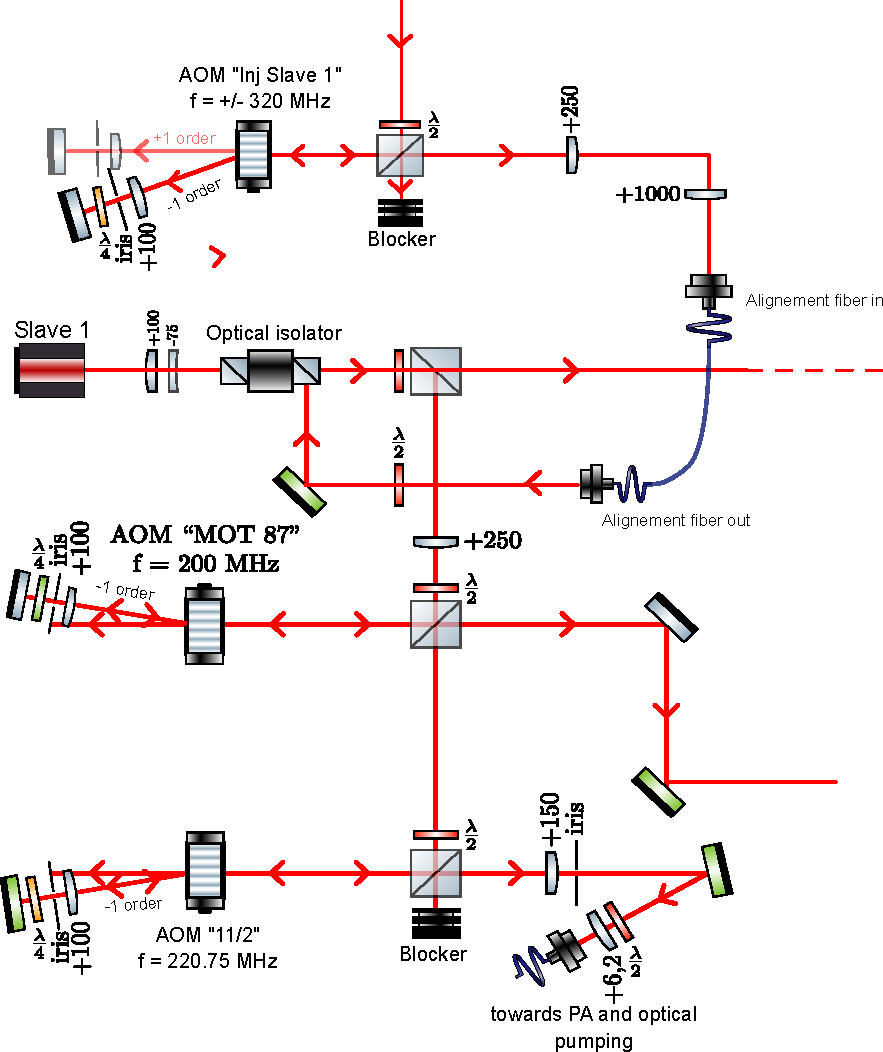
\includegraphics[width=0.9\linewidth]{Chapitres/Engineering highly entangled system of photoassociated 87Sr atoms/images/Schemas_optiques/zoom_red_chain_beating.pdf}
    \caption[]{Zoom on the section of the red chain dedicated to the PA process. The
frequency for both laser configurations is tuned by ”AOM Inj Slave 1”, adjusted by
”AOM 11/2” before being sent to the atoms.}
    \label{zoom red chain battement}
\end{figure}

\subsection{Verification of the molecular nature of the lines}
\subsubsection{dN/dt decay interpretation}
Before presenting the molecular lines obtained for $^{87}Sr$ I want to discuss the reliability of the $dN/dt$ test to identify the nature of the losses.
While the two slopes are usually a signature of two-body losses I observed the same behavior for the atomic resonance obtained with the red diode noise at 
6 MHz as visible in \ref{exp decay 6 MHz noise} in dark purple. This experiment has been obtained on a red detuned signal from $F=11/2$ hyperfine state of $^{87}$Sr.
The atoms have been evaporated during $500$ ms, recompressed and illuminated during $T = 2000$ms. In this figure the atom decay is clearly well described 
by equation \ref{one and two body losses equation} and presents a change of slope around 3s: the fit of this data leads to a misinterpretation of the collision nature. 
The same data in the absence of the PA laser plotted in the same figure shows a linear behavior on the atomic decay. As presented in 3.3.2.2 the exponential 
decay test is done in atomic resonance: this measurement is not reliable to identify with certainty the nature of the losses while no molecule has been enhanced on this
experiment.
\begin{figure}[H]
    \centering
    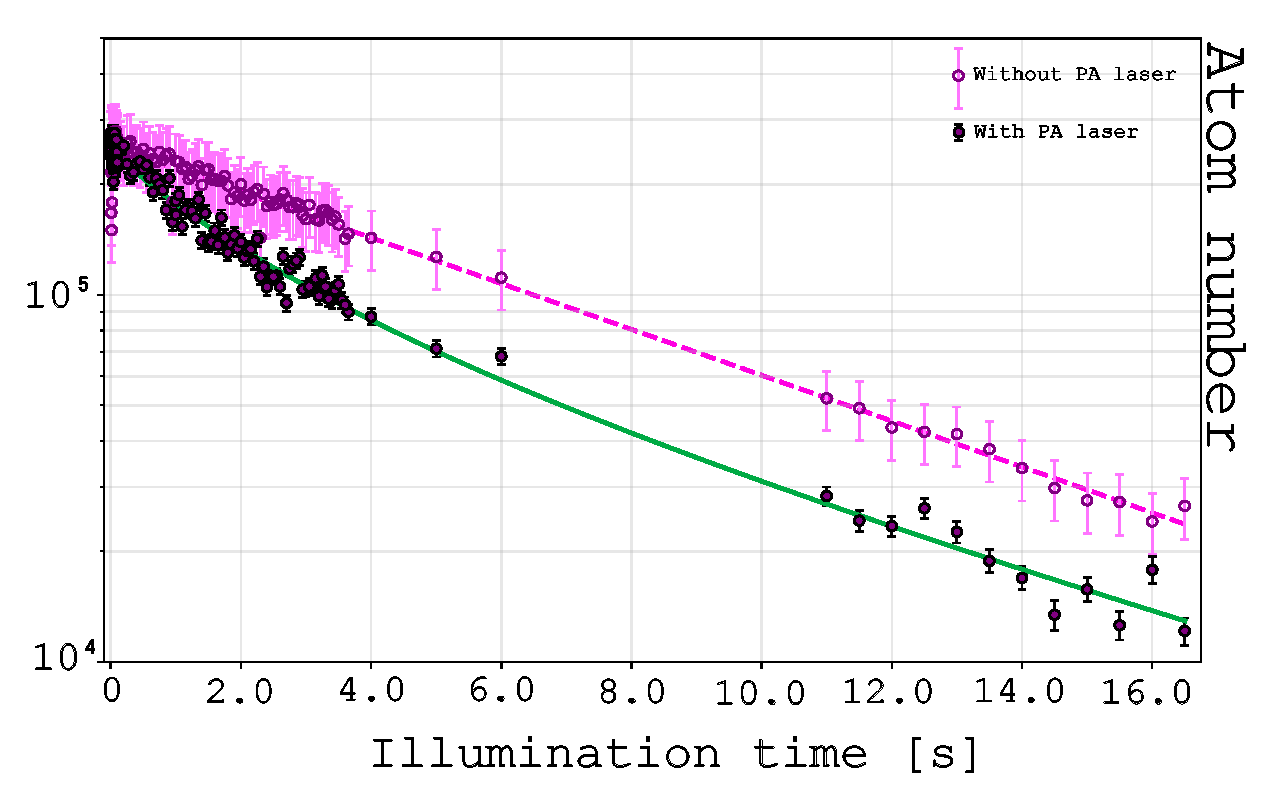
\includegraphics[width=1\linewidth]{Chapitres/Engineering highly entangled system of photoassociated 87Sr atoms/images/87Sr/data16_exp_bruit_6MHz.pdf}
    \caption[Evolution of the atom number as a function of the illumination time at $f = -6$~MHz]{Evolution of the atom number (on a logarithmic scale) as a function of the illumination time, measured at a fixed laser detuning of $f = -6$~MHz from the atomic resonance (see Section 3.2.3.5). Filled circles represent the data in the presence of the photoassociation (PA) laser, adjusted with the fit function (Eq.~\ref{eq:final_fit}) accounting for combined one- and two-body losses. Open circles display the reference measurement at the same frequency in the absence of the PA laser. The distinct decay behaviors observed between the two datasets highlight that relying solely on a single $dN/dt$ decay measurement is insufficient to unambiguously characterize the loss mechanisms.}
    \label{exp decay 6 MHz noise}
\end{figure}
It appears that for non-recompressed gas it is possible to still have thermalization when the evaporation is not well optimized and 
that affects the two-body losses rate. For recompressed gas as in \ref{exp decay 6 MHz noise} collisions keep occuring for atoms contained 
in a smaller volume which explains the slope break on the plot.

\subsubsection{Temperature as an ultimate proof}
A last trustworthy test is the measurement of the temperature of the gas: when PA occurs we expect the gas to be hotter. The coldest atoms
at the bottom of the trap are most likely to photoassociate. Then the resting atoms redistribute by elastic collisions leading to a hotter gas
with a mean temperature per atom increased.

Figure \ref{temp 6MHz noise} is a representation of the temperature of the gas during the same experiment as \ref{6MHz noise red detuned}.
This plot shows a linear increase of the temperature coming from the direct increase of illumination time: there is no exponential behavior of 
this curve as expected.

\begin{figure}[H]
    \centering
    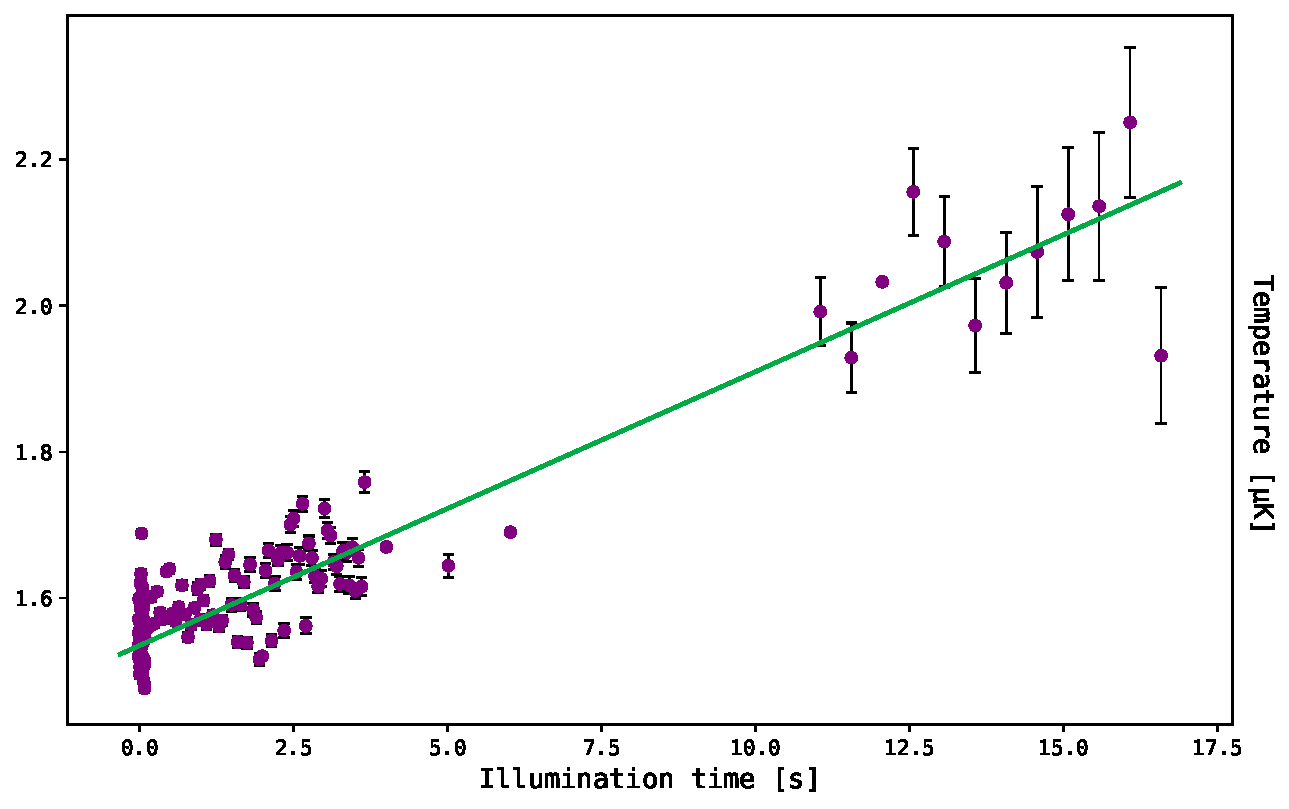
\includegraphics[width=1\linewidth]{Chapitres/Engineering highly entangled system of photoassociated 87Sr atoms/images/87Sr/temp_data_16.pdf}
    \caption[]{Temperature of the gas during the experiment described in \ref{6MHz noise red detuned} where we observe a number of atoms decaying 
    with a two-body loss-like behavior while it is not the case. The temperature of the gas does not show any increase which is a proof of the elastic
    collisions only and the absence of molecule formation.}
    \label{temp 6MHz noise}
\end{figure}

The cloud temperature is derived assuming an isotropic thermal velocity distribution. During time-of-flight (TOF), the cloud undergoes isotropic ballistic expansion, where the Gaussian width $\sigma_y$ measured along a given axis evolves as:
\begin{equation}
    \sigma_y^2 = \sigma_{0,y}^2 + v_{\text{th}}^2 \, \text{TOF}^2
\end{equation}

where $\sigma_{0,y}$ is the \textit{in-situ} RMS width of the gas in the optical dipole trap (ODT) intersection, and $v_{\text{th}}$ is the thermal velocity. 

Assuming a Maxwell-Boltzmann velocity distribution, the equipartition theorem links the thermal velocity to the isotropic temperature $T$ along each degree of freedom via $\frac{1}{2} m_{\text{at}} v_{\text{th}}^2 = \frac{1}{2} k_B T$. The temperature is thus extracted from the Gaussian spatial width $\sigma_y$ measured on the absorption image:
\begin{equation}
    T = \frac{m_{\text{at}} \left(\sigma_y^2 - \sigma_{0,y}^2\right)}{k_B \, \text{TOF}^2}
\end{equation}
Assuming independent uncertainties on both the \textit{in-situ} size $\sigma_{0,y}$ and the expanded size $\sigma_y$, error propagation in quadrature yields:
\begin{equation}
    \delta T = \frac{2 m_{\text{at}}}{k_B \, \text{TOF}^2} \sqrt{\left(\sigma_y \delta \sigma_y\right)^2 + \left(\sigma_{0,y} \delta \sigma_{0,y}\right)^2}
\end{equation}

\subsubsection{Molecular lines on $^{87}Sr$}
%----------------------------------------------------------
% LINE 1: 259.01 MHz
%----------------------------------------------------------


\paragraph{Line at $-259.01$ MHz}
I did find the closest molecular state red detuned from the atomic resonance at $f_1 = -259.01\pm 0.12$: it has been obtained for illumination time of t = 1000~ms on a 
recompressed gas at intensity $I = 19$~W/cm$^2$.
The lorentzian shape of the data \ref{subfig:259MHz_spectrum} (see 3.2.3.2) reveals a surprising measured linewidth of $\Gamma = 2.53 \pm 0.17$~MHz with a maximized contrast
of half of the atom number at resonance. \\

Fig.\ref{subfig:259MHz_temp} is a measurement of the temperature of the cloud from the same experiment that should validate the molecular nature of the collisions. While one
expect an increase of the temperature at the center frequency of the molecular line the temperature appears to increase for about 0.5~$\mu$K symmetrically with the resonance, 
where the width of the lorentzian fit of the resonance is marked by the green dashed lines.\\


The analysis of the resonance is completed by the exponential decay observation in \ref{subfig:274MHz_exp}: the data is fitted by the function demonstrated in \ref{eq:final_fit} with 
an interpolation of the temperature during the illumination time with a unique value of $\beta(T)$ for each point. Figure \ref{subfig:274MHz_temp} shows a lot of fluctuations on the temperature
that is directly impacting the shape of the atomic number decay over the time. 

\begin{figure}[H]
    \centering
    \begin{subfigure}{0.8\linewidth}
        \centering
        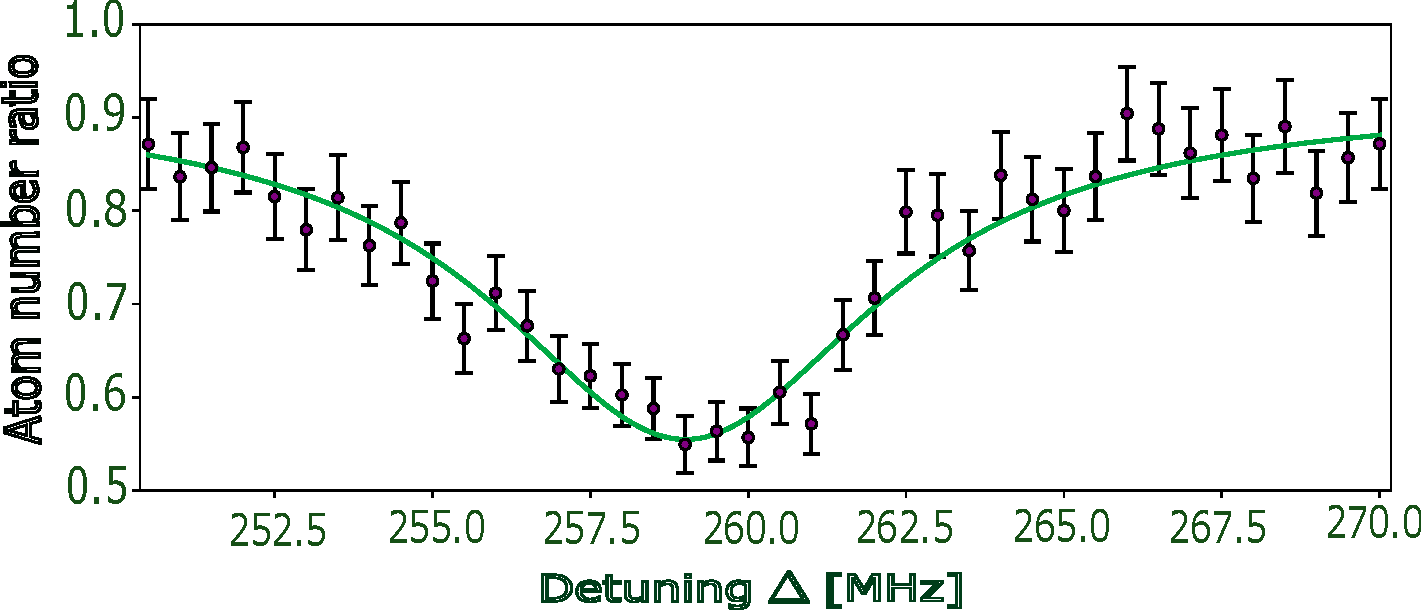
\includegraphics[width=1\linewidth]{Chapitres/Engineering highly entangled system of photoassociated 87Sr atoms/images/87Sr/normalisation_data195.pdf}
        \caption{Resonance spectrum at $259.01 \pm 0.12$ MHz ($I = 19$ W/cm$^2$ for t = 1000~ms).}
        \label{subfig:259MHz_spectrum}
    \end{subfigure}

    \begin{subfigure}{0.8\linewidth}
        \centering
        % TODO: add temperature figure for 259 MHz line
        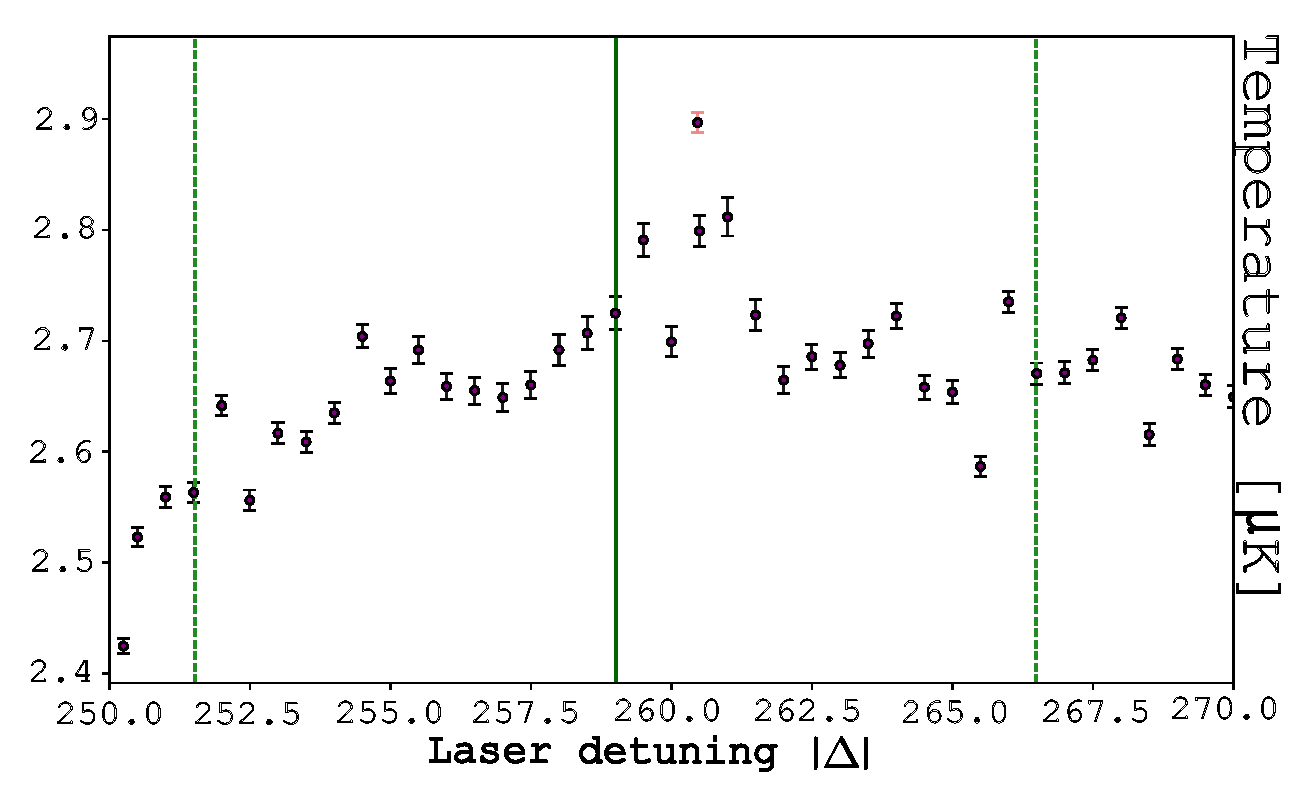
\includegraphics[width=1\linewidth]{Chapitres/Engineering highly entangled system of photoassociated 87Sr atoms/images/87Sr/temp_data_195.pdf}
        \caption{Temperature of the gas at the $259.01$ MHz resonance.}
        \label{subfig:259MHz_temp}
    \end{subfigure}
    
\begin{subfigure}{0.8\linewidth}
        \centering
        % TODO: add temperature figure for 259 MHz line
        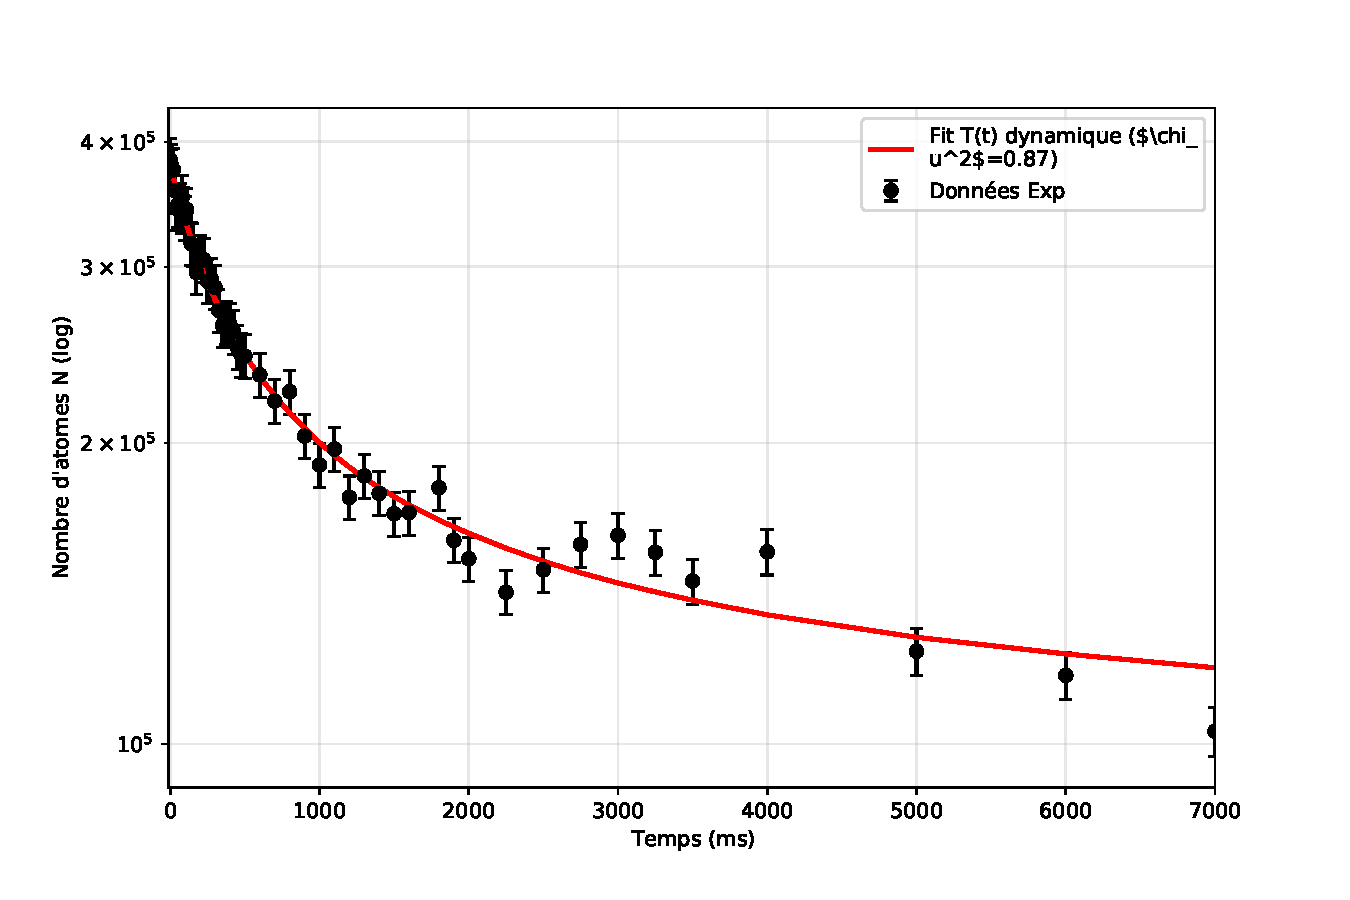
\includegraphics[width=1\linewidth]{Chapitres/Engineering highly entangled system of photoassociated 87Sr atoms/images/87Sr/data247_exp_.pdf}
        \caption{ at the $259.01$ MHz resonance.}
        \label{subfig:259MHz_temp}
    \end{subfigure}

    \caption{Characterization of the molecular line at $259.01 \pm 0.12$ MHz in $^{87}$Sr ($I = 19$ W/cm$^2$). 
    All detunings are measured from the $^{87}$Sr atomic resonance.}
    \label{fig:line_259MHz}
\end{figure}
%----------------------------------------------------------
% LINE 2: 274.83 MHz
%----------------------------------------------------------
\paragraph{Line at $276.83$ MHz}
The second line detected is at $f_2 = -276.83\pm 0.03$ MHz from the atomic resonance plotted in \ref{subfig:274MHz_spectrum}. The gas prepared of density
$2\times 10^{13}$~atoms/cm$^3$ was evaporated in the crossing and illuminated for 1000~ms.
in reservoir and dimple
Once again the linewidth measured $\Gamma = 7.48 \pm 0.77$ is surprisingly large. The points out of the fit could come from a delocking laser or 
simply a mis-fitting of the gaussian shape of the gas. \\

The measurement of the temperature \ref{subfig:274MHz_temp} is almost maximum at the center of the resonance but shows an unexplained oscilation 
just after of about $0.1~\mu$K around $1.52~\mu$K.\\

The exponential decay of this resonance, as for the previous one, has first been tested with an invariant temperature which gave an unsuccessful fit \ref{subfig:274MHz_exp} 
with an associated really low value of $l_{opt}/I = (2.6 \pm 0.9)\times 10^{-6}~a_0/(W/cm^2)$.\\


Then I solved the misfitting by considering the $\beta$ factor dependant with the temperature since the gas is hotter when photoassociated and the plot of the 
temperature shows lots of fluctuations. 

The interpolation of the temperature during the illumination time is then used to fit the data with a unique value of $\beta(T)$ for each point.

\begin{figure}[H]
    \centering
    \begin{subfigure}{0.8\linewidth}
        \centering
        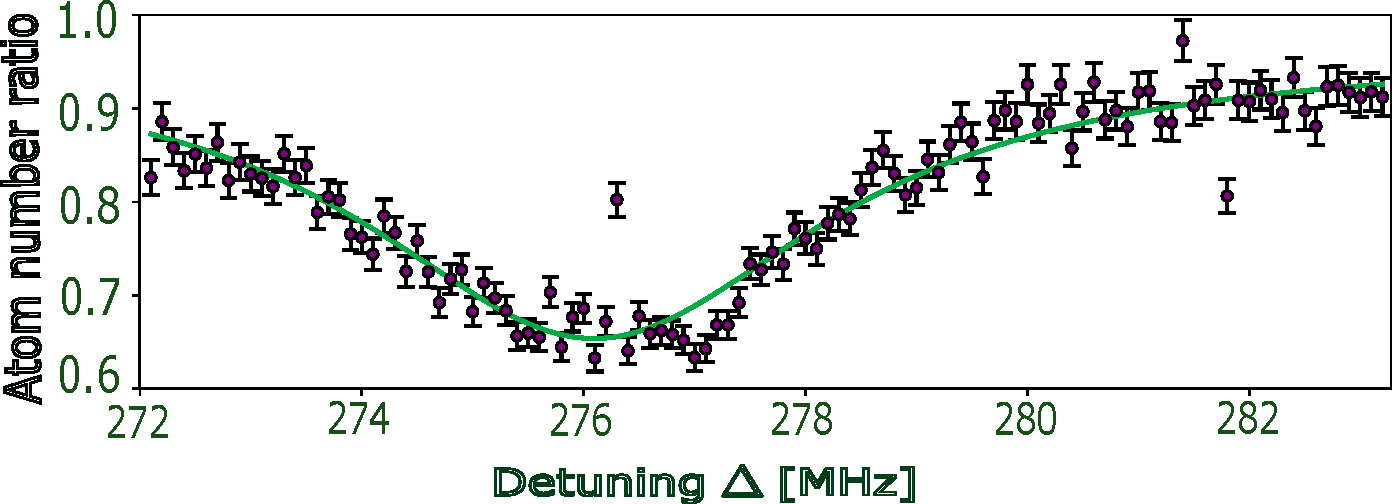
\includegraphics[width=1\linewidth]{Chapitres/Engineering highly entangled system of photoassociated 87Sr atoms/images/87Sr/data171.pdf}
        \caption{Resonance spectrum at $276.83 \pm 0.03$ MHz ($I = 5.2$ W/cm$^2$ for t = 1000~ms).}
        \label{subfig:274MHz_spectrum}
    \end{subfigure}

    \begin{subfigure}{0.8\linewidth}
        \centering
        % TODO: temperature figure for 274.83 MHz line not yet added
        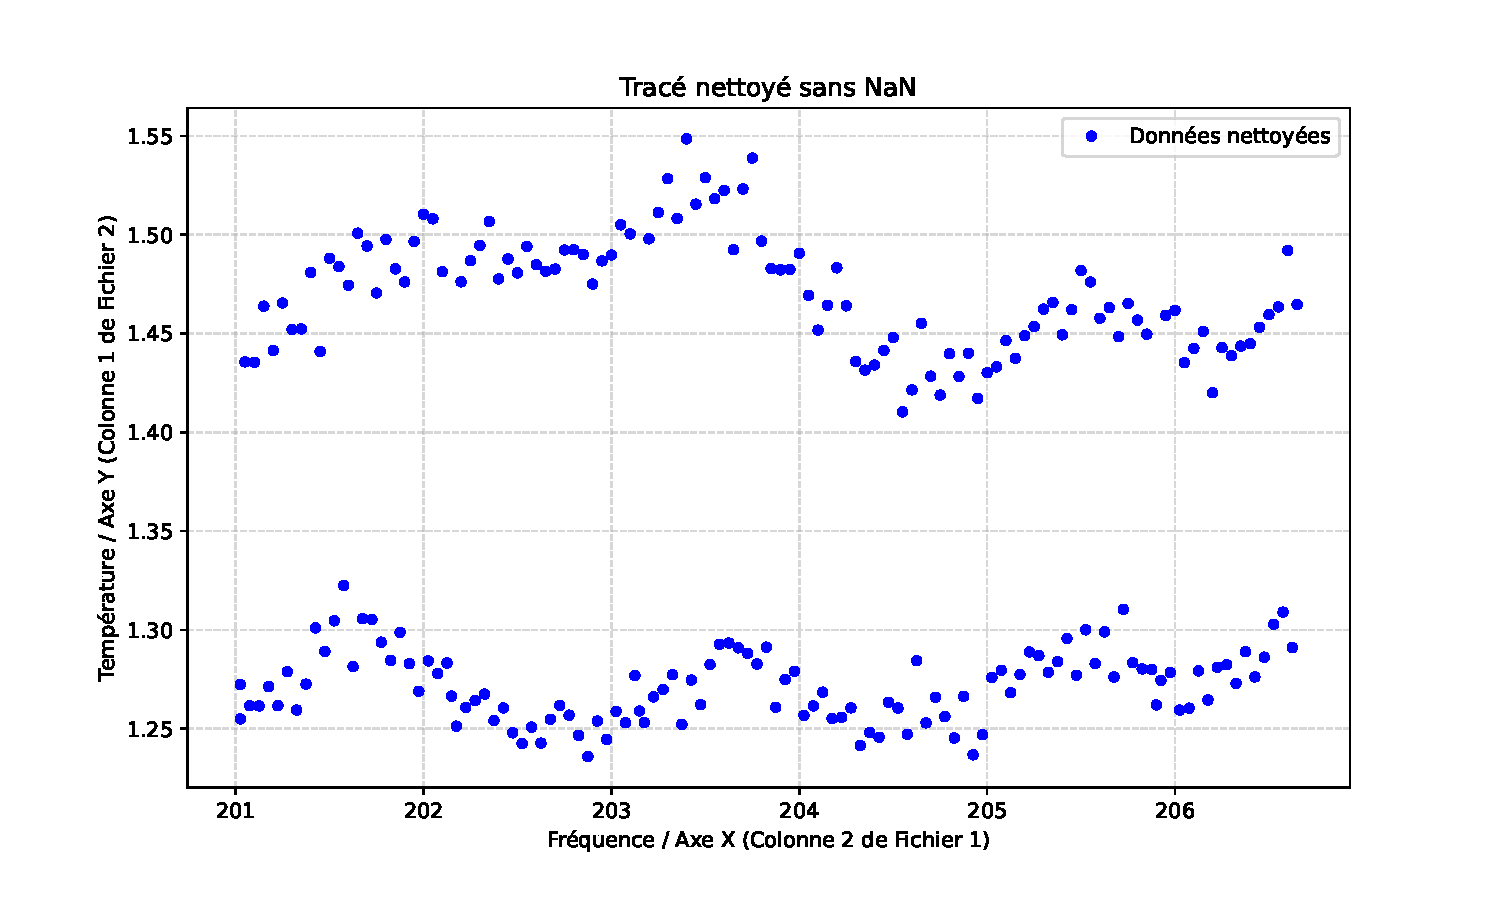
\includegraphics[width=1\linewidth]{Chapitres/Engineering highly entangled system of photoassociated 87Sr atoms/images/87Sr/temp_data_171.pdf}
        \caption{Temperature of the gas at the $276.83$ MHz resonance (figure to be added).}
        \label{subfig:274MHz_temp}
    \end{subfigure}

    \begin{subfigure}{0.8\linewidth}
        \centering
        % TODO: temperature figure for 274.83 MHz line not yet added
        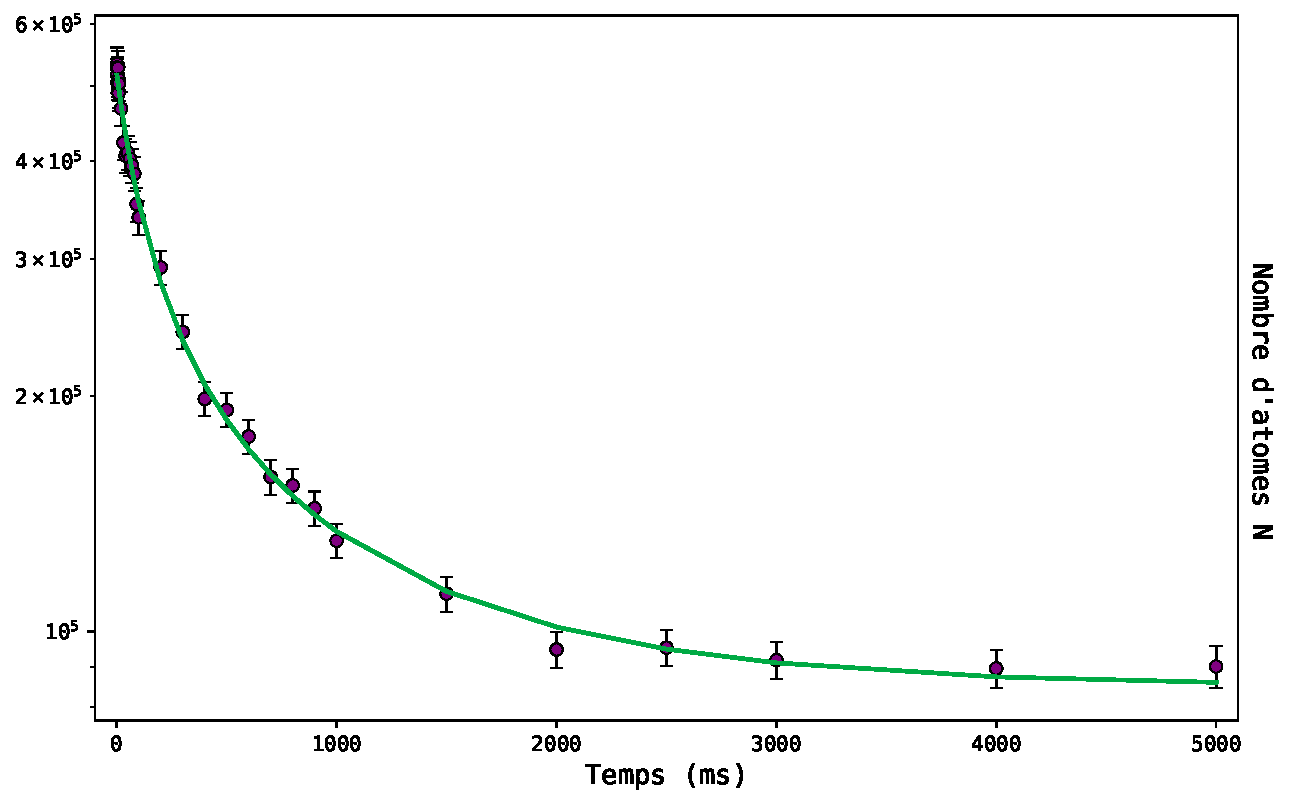
\includegraphics[width=1\linewidth]{Chapitres/Engineering highly entangled system of photoassociated 87Sr atoms/images/87Sr/data190_exp.pdf}
        \caption{}
        \label{subfig:274MHz_exp}
    \end{subfigure}

    % NOTE: no exponential decay figure available for this line
    \caption{Characterization of the molecular line at $276.83 \pm 0.03$ MHz in $^{87}$Sr ($I = 5.2$ W/cm$^2$). 
    No exponential decay measurement is available for this line.
    All detunings are measured from the $^{87}$Sr atomic resonance.}
    \label{fig:line_276MHz}
\end{figure}

%----------------------------------------------------------
% LINE 3: 375.74 MHz
%----------------------------------------------------------
\paragraph{Line at $375.74$ MHz}
The last measured molecular line at $f_3 = 375.74 \pm 0.48$\,MHz is obtained for a recompressed gas illuminated during \qty{1000}{ms} with an intensity $I = 5.6$\,W/cm$^{2}$.
It has a really low contrast and still a large linewidth of $\Gamma = 10.96 \pm 2.68$~MHz.
The temperature measurement in \ref{subfig:375MHz_temp} shows a frank slope change between the resonance and the red detuned frequencies where it decreases
to $\Delta T = 200$~nK. The temperature being mostly constant during the entire molecular resonance $dN/dt$ measurement \ref{subfig:375MHz_exp} is well described
by the fitting function \ref{eq:final_fit} valid for $\beta$ independant on T. \hl{slopes ?}

\begin{figure}[H]
    \centering
    \begin{subfigure}{0.75\linewidth}
        \centering
        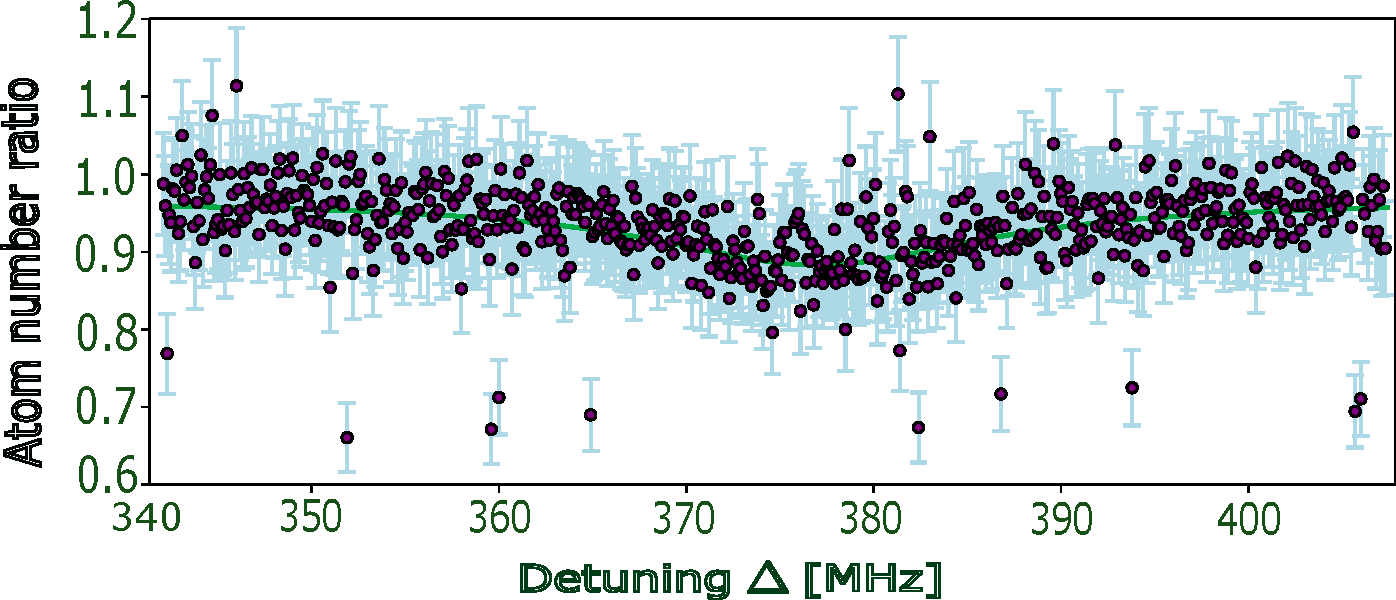
\includegraphics[width=1\linewidth]{Chapitres/Engineering highly entangled system of photoassociated 87Sr atoms/images/87Sr/normalisation_data184.pdf}
        \caption{\hl{attention premier trait 360 au lieu de 340} Resonance spectrum at $375.74 \pm 0.48$ MHz ($I = 5.6$ W/cm$^2$ for t = 1000~ms).}
        \label{subfig:375MHz_spectrum}
    \end{subfigure}

    \begin{subfigure}{0.75\linewidth}
        \centering
        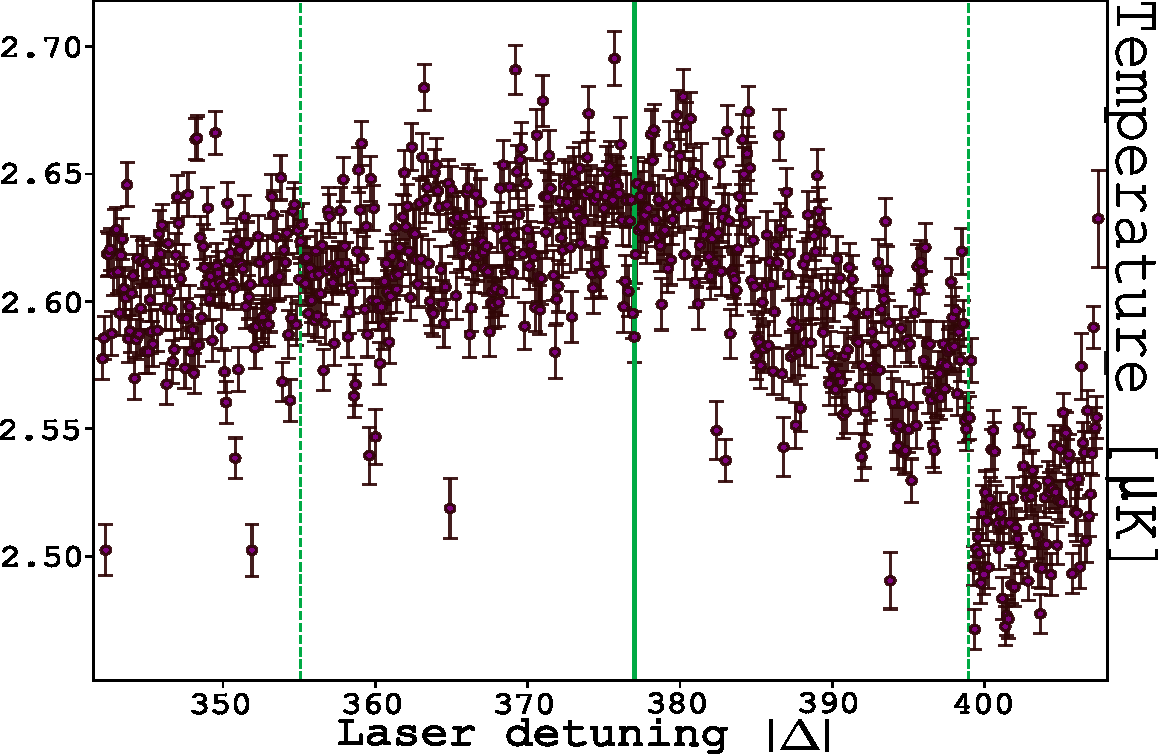
\includegraphics[width=1\linewidth]{Chapitres/Engineering highly entangled system of photoassociated 87Sr atoms/images/87Sr/temp_data_184.pdf}
        \caption{Temperature of the gas at the $375.74$ MHz resonance.}
        \label{subfig:375MHz_temp}
    \end{subfigure}

    \begin{subfigure}{0.75\linewidth}
        \centering
        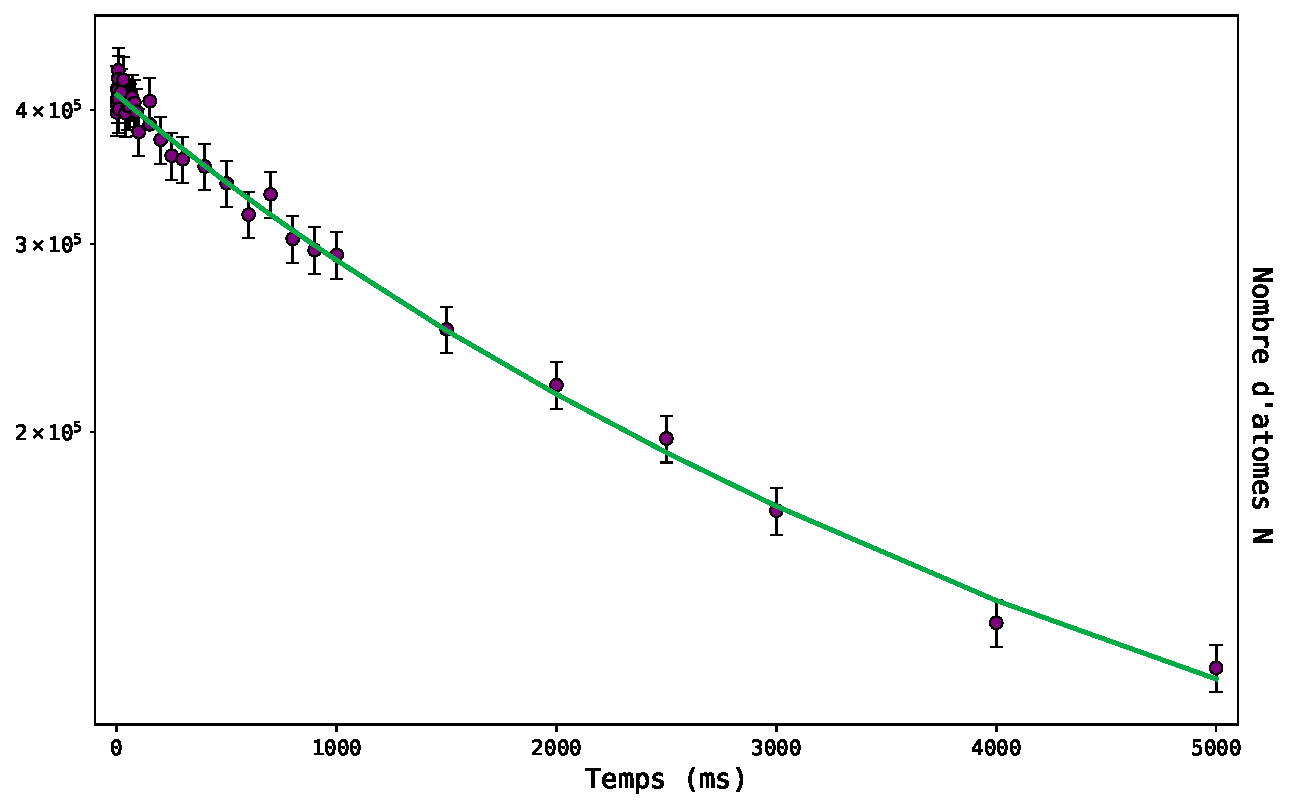
\includegraphics[width=1\linewidth]{Chapitres/Engineering highly entangled system of photoassociated 87Sr atoms/images/87Sr/data_194_exp.pdf}
        \caption{Exponential decay (one- and two-body losses) at the $375.74$ MHz resonance.}
        \label{subfig:375MHz_exp}
    \end{subfigure}
    \caption{Characterization of the molecular line at $375.74 \pm 0.48$ MHz in $^{87}$Sr ($I = 5.6$ W/cm$^2$ for t = 1000~ms). 
    All detunings are measured from the $^{87}$Sr atomic resonance.}
    \label{fig:line_375MHz}
\end{figure}

The exponential decay of the second molecular line at $f = 276.83$ MHz is presented in figure \ref{subfig:276MHz_temp}: 
% TODO: update this sentence once the exponential decay for the 276.83 MHz line is available.
\begin{table}[htbp]
\centering
\caption{Summary of fit parameters and experimental conditions for data series 171, 195, and 184.}
\label{tab:summary_fits_PA_final}
\small
\renewcommand{\arraystretch}{1.2} % Ajoute un peu d'espace vertical entre les lignes
\begin{tabular}{l c c c}
\hline \hline
\textbf{Freq. $f$ (MHz)} & \textbf{$259.01 \pm 0.12$} & \textbf{$276.83 \pm 0.03$} & \textbf{$375.74 \pm 0.48$} \\ 
\hline
Depth & $-0.307 \pm 0.010$ & $-0.364 \pm 0.019$ & $-0.083 \pm 0.009$ \\
Width (MHz) & $2.53 \pm 0.17$ & $7.48 \pm 0.77$ & $10.96 \pm 2.68$ \\
Time $t$ (ms) & 1000 & 1000 & 1000 \\ 
Intensity for resonance $I$ (W/cm$^2$) & 19 & 5.2 & 5.6 \\
\hline
Intensity $I$ for $l_{opt}$ (W/cm$^2$) & 19 & 31 & 19 \\
$l_{opt}/I$ ($a_0/(W/cm^2)$) & $(6.11\pm 3.34)\times 10^{-1}$ & $ (5.2 \pm 0.4)\times 10^{-1}$ & $(3.24 \pm 2.25)\times 10^{-2}$ \\ 
\hline \hline
\end{tabular}
\end{table}


\noindent\textbf{Defining $l_{\text{opt}}$}\\
There are two ways to determine the optical length. 
One is to use the Lorentzian fit of the resonance. Following the formulation from \cite{zelevinsky_narrow_2006}, the inelastic two-body loss rate coefficient is expressed as:
\begin{equation}
    K_2(\Delta) = \frac{4\pi\hbar}{\mu} \frac{\Gamma_{\text{mol}}^2 l_{\text{opt}}}{\left(\frac{E}{\hbar} + 2\pi\Delta\right)^2 + \frac{(\Gamma_{\text{stim}} + \Gamma_{\text{mol}})^2}{4}}
    \label{eq:zelevinsky_K2}
\end{equation}
where $\mu$ is the reduced mass $m_{at}/2$, $\Gamma_{\text{mol}}$ is the natural molecular linewidth, and $\Gamma_{\text{stim}}$ is the light-induced stimulated width. 

Experimentally, the loss profile is fitted using a standard empirical Lorentzian function where the frequency offset is explicitly written to match the resonance condition:
\begin{equation}
    f(\Delta) = \frac{A}{1+\left(\frac{\Delta + \frac{E}{2\pi\hbar}}{\Gamma_{\text{fit}}/2}\right)^2} = \frac{A (\Gamma_{\text{fit}}/2)^2}{(\Gamma_{\text{fit}}/2)^2 + \left(\Delta + \frac{E}{2\pi\hbar}\right)^2}
    \label{eq:lorentzian_fit_standard}
\end{equation}
where $A$ is the peak amplitude and $\Gamma_{\text{fit}}$ is the full-width at half-maximum (FWHM) extracted by the fitting software.

By dividing both the numerator and denominator of Eq.~\ref{eq:zelevinsky_K2} by $(2\pi)^2$, the identity with Eq.~\ref{eq:lorentzian_fit_standard} becomes direct and allows us to map the physical parameters to our fit observables:
\begin{align}
    \Gamma_{\text{fit}} &= \frac{\Gamma_{\text{stim}} + \Gamma_{\text{mol}}}{2\pi} \\[1.5ex]
    A &= \frac{4\hbar}{\pi\mu} \frac{\Gamma_{\text{mol}}^2 l_{\text{opt}}}{\Gamma_{\text{fit}}^2}
\end{align}

Remarkably, the product of the amplitude and the square of the linewidth eliminates the temperature-dependent broadening terms. The optical scattering length $l_{\text{opt}}$ can therefore be straightforwardly extracted from the experimental fit parameters via:
\begin{equation}
    l_{\text{opt}} = \frac{\pi m_{at}}{8\hbar\Gamma_{\text{mol}}^2} \times \left( A \cdot \Gamma_{\text{fit}}^2 \right)
\end{equation}

The second way to define $l_{opt}$ is straightforward : $dN/dt$ fit gives an estimation of $K_2$ that is related with $l_{opt}$ as $K_2 = \frac{16 h}{m_{at}l_{opt}}$.
\hl{calculs lopt avec les valeurs d'ammplitude NON NORMALISEES car valeurs actuelles relevées pour 87 fausses }
\hl{Ajouter commentaires sur le calcul de T et estimation incertitude}

\textbf{PA lines found on $^{87}Sr$}\\
These results show multiple surprising behaviors of our atoms :

\begin{itemize}
    \item First, we have not been able to detect two-body losses before $259.01$ MHz which is surprising taking into acount the expect frequency ranges on $87$ isotope from mass scaling discussion of \cite{borkowski_mass_2014}.
    \item Then we hardly exceed $30\%$ of loss: all three datas present small depths from $8.3\pm 0.9 \%$ to $36.4\pm 1.9 \%$ for intensites greater than many experiments like \cite{zelevinsky_narrow_2006} and similar atomic densities. 
    \item In addition the linewidth of each line is large : $2.53 \pm 0.17$, $7.48 \pm 0.77$ MHz and $10.93 \pm 2.68$ MHz while we expect $\Gamma = \gamma_{mol} \simeq 2\times \gamma_{at} \simeq 15$ kHz.
\end{itemize}


The plots of molecular lines added to the really low estimated $l_{opt}$ values for high intensity expose multiple unexpected behaviours.\\
In the next subsection I will discuss the possible interpretation of these caracteristics.

\subsection{Interpretation of low contrast}
The surprising low number of the $^{87}Sr$ PA lines coupled to the large width and low strength of the lorentzian shape have been observed in \cite{franzen_intercombination_2023}. where $^{87}Rb^{170}Yb$ bi-alkali molecules are photoassociated on the intercombination line. 
Only two spectroscopic lines have been observed with a low contrast while the intensity of the laser reaches $I = 40~$mW/cm$^2$ corresponding to a two-body loss rate $\beta = 5\times 10^{-14}~$cm$^3$/s corresponding to a really low optical length.\\

Authors give two interpretations for this result : the first one is the strong dipole at low internuclear distance coming from the rubidium potentials, leading to atomic decay to $^1S_0$. Nevertheless this effect is estimated to be less than 10\% probable.  \\
The second interpretation is the predissociation process illustrated in Fig.\ref{predissociation}. Two free atoms from potential A are photoassociated to a vibrationnal state of a molecular potential B. Atomic potential C crosses potential B above its dissociation limit which 
creates a coupling between the two potentials (\cite{mukherjee_feshbach_2022}). In the case of $^{87}Sr$ this potential is one of the hyperfine structure of the $^3P_J$ state. The bound atoms then decay to the continuum of the potential C that impacts the lifetime of the excited
molecular state as 
\begin{equation}
    \Gamma_{eff} = \Gamma_{stim} + \Gamma_{predissociation} + \Gamma_{mol}
\end{equation} 

with $\Gamma_{predissociation} \propto \rho(\epsilon_f)$ where $\rho(\epsilon_f)$ is the density of states of the potential C at the energy of the molecular state. The predissociation process is then a loss channel for the molecular state that decreases the lifetime of the molecule and increases its linewidth. 


In \ref{fig:pa-ytterbium-potentials} the curves do not seem to be affected by the predissociation from the linewidth values. We were thinking that PA on the lowest
hyperfine state as for $Yb$ would avoid this effect but the data on $^{87}Sr$ show the contrary: for a reason we ignore this atom is affected by this process but the 
$Yb$ with hyperfine structure is not.

\begin{figure}[H]
    \centering
    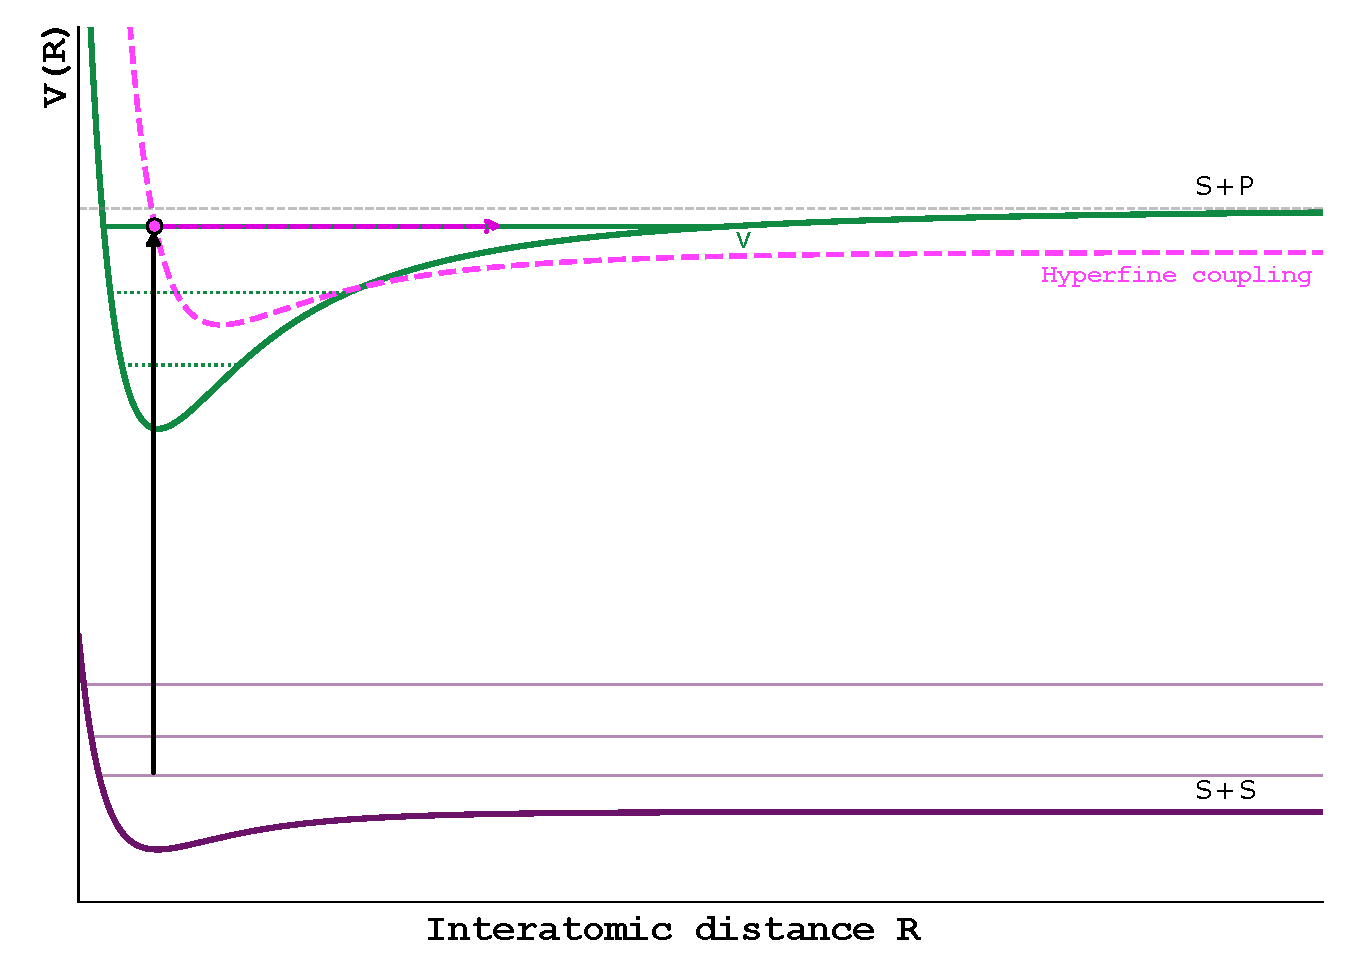
\includegraphics[width=0.5\linewidth]{Chapitres/Engineering highly entangled system of photoassociated 87Sr atoms/images/Figures_pour_theorie/predissociation.pdf}
    \caption[predissociation]{Scheme of predissociation which is a phenomenon that occurs when dissociation limit of an excited molecular potential
C is under the closed channel of the excited molecule of potential B. Then the $\nu_ B$ state is coupled to a density of states of potential
C that modifies the linewidth $\Gamma_mol$ of the molecular state}
    \label{predissociation}
\end{figure}
Changing the polarization of the PA laser could change the coupling strength with the atomic continuum.
Same as for the magnetic field that could change the energy difference between the hyperfine states and so decrease the density of states. Both of these possibilities have been tested following this work I presented but no significant change has been observed on the linewidth and the contrast of the molecular lines.\\
\subsubsection{Coupling to more energetic state from the IR}
ODT can be a distructive source of PA process if it is resonant with high energy levels at $\lambda = 1064$nm from the target state
of the first molecular excited state.
The experimental sequence of \ref{sequence chirp} implements a chopping of optical trap in opposite phase with PA laser that suppresses eventual coupling to much higher levels.

\begin{figure}[H]
    \centering
    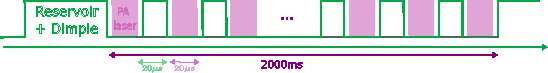
\includegraphics[width=1\linewidth]{Chapitres/Engineering highly entangled system of photoassociated 87Sr atoms/images/Figures_pour_theorie/sequence_chopping.pdf}
    \caption[sequence chirp]{Experimental sequence of IR and PA laser chopping to cancel possible coupling to higher energy levels around 
    $\lambda = 1064nm$ that would destruct or decrease collision process. The RF signal of ODT and Raman AOMs is modulated by a GBF at 
    frequency $25$ kHz in opposite phaseso the atoms in the trap are not lost during the $100\mu$ s falling time when photoassociated.}
    \label{sequence chirp}
\end{figure}

\subsection{Conclusion and outlook}
To conclude on this chapter I started to present theoretical aspect of PA process by introducting fundamental material such as scattering length, optical length, atoms evolution time for two-body collisions... Then I presented the experimental results on $^{88}Sr$ on intercombination line as a reference to experimentally characterize the process. This chapter ends up with the measurement of molecular lines on an unpolarized gas of $^{87}Sr$ that comes with low contrast and wide linewidth, explained by predissociation process higly present for numerous molecular potentials such as $^{87}Sr$ being an atom with hyperfine structure.\\

Predissociation could be proved by implementing again the optical pumping on the experiment: the number of potentials will decrease and the density of states $\rho(\epsilon_f)$ also. Then the contrast of the molecular lines and their associated linewidth will be improved.\\
Optical pumping tests have already been operated to enhance SU(2) gas with maximum value $m_F = 9/2$ and $m_F = -9/2$ in order to have the maximum value of $T, m_T$ and 


%The last part of this work is to test the final Dicke state we expect to engineer by this PA experiment. A way to test it is to create Ramsey interferometers -as in section 2 of this thesis- on a controllable Hilbert space of low dimension.


%\subsubsection{Node of wavefunction for some vibrational states}

%Vibrational states whose wavefunction has a node at the Condon radius cannot be excited by the PA laser.
%In figure \ref{fig:PA_concept} the wavefunction of the second bound state crosses the molecular potential
%at a node. It means that if we try to PA atoms from the free atoms to this molecular state we would not see
%any atom loss.
